
\chapter{Introduction}
\label{sec:Introduction}

\label{sub:figures}
\begin{figure}[ht]
	\begin{center}
		\begin{subfigure}[b]{0.33\textwidth}
			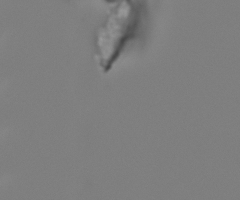
\includegraphics[width=\textwidth]{thesis-template-master/images/(1095).png}
			\caption{Debris}
			\label{fig:Debris}
		\end{subfigure}
		\begin{subfigure}[b]{0.33\textwidth}
			\reflectbox{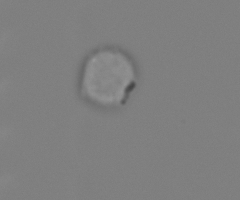
\includegraphics[width=\textwidth]{thesis-template-master/images/(635).png}}
			\caption{Out of Focus}
			\label{fig:Out of Focus}
		\end{subfigure}
		\begin{subfigure}[b]{0.33\textwidth}
			\reflectbox{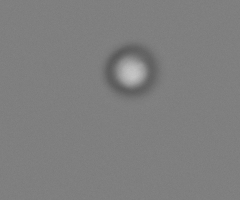
\includegraphics[width=\textwidth]{thesis-template-master/images/(1672).png}}
			\caption{Lighting Artifacts}
			\label{fig:Lighting Artifacts}
		\end{subfigure}
		\begin{subfigure}[b]{0.33\textwidth}
			\reflectbox{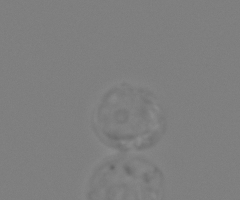
\includegraphics[width=\textwidth]{thesis-template-master/images/(1112).png}}
			\caption{Outside FOV}
			\label{fig:Outside FOV}
		\end{subfigure}
		\begin{subfigure}[b]{0.33\textwidth}
			\reflectbox{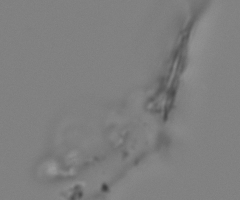
\includegraphics[width=\textwidth]{thesis-template-master/images/(1684).png}}
			\caption{Contaminated}
			\label{fig:Contaminated}
		\end{subfigure}
		\begin{subfigure}[b]{0.33\textwidth}
			\reflectbox{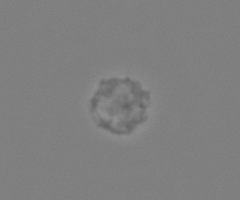
\includegraphics[width=\textwidth]{thesis-template-master/images/hd3 (56).png}}
			\caption{Good Cell}
			\label{fig:Good Cell}
		\end{subfigure}
	\end{center}
	\caption{Six Typical Cell images on original Sezary Syndrome data set. Only Good Cell can provide useful Morphology characteristics for further classification.}
	\label{fig:lennas}
\end{figure}
Sezary Syndrom is an aggressive form of cutaneous T-cell lymphoma that is characterized by presence of tumor T-cells with abnormal nucleus morphology in the peripheral blood. The easy and precise detection of malignant cells in the blood of patients with Sezary Syndrome is of important diagnostic, prognostic and therapeutic value, and is essential for disease monitoring under treatment\cite{b6}\cite{b7}. The severe limitations of manual microscopic identification of tumor T-cells have led to the implementation of flow cytometry-based diagnostic assays. Currently, the loss of cell surface markers, such as CD26, CD27 and CD7, on malignant T lymphocytes remains one of the most consistent features and is routinely used in the diagnostic workup \cite{b12}, although their specificity and especially sensitivity, must be interpreted with caution \cite{b11}. We plan to circumvent the challenges involving the definition of molecular diagnostic markers and rather aim at re-surging morphology-based diagnosis of hematological malignancies through an automated procedure, integrating imaging flow cytometry and deep learning as a route to, ultra-high throughput and sensitive diagnosis.
 
\label{sub:figures}
\begin{figure}[ht]
	\begin{center}
	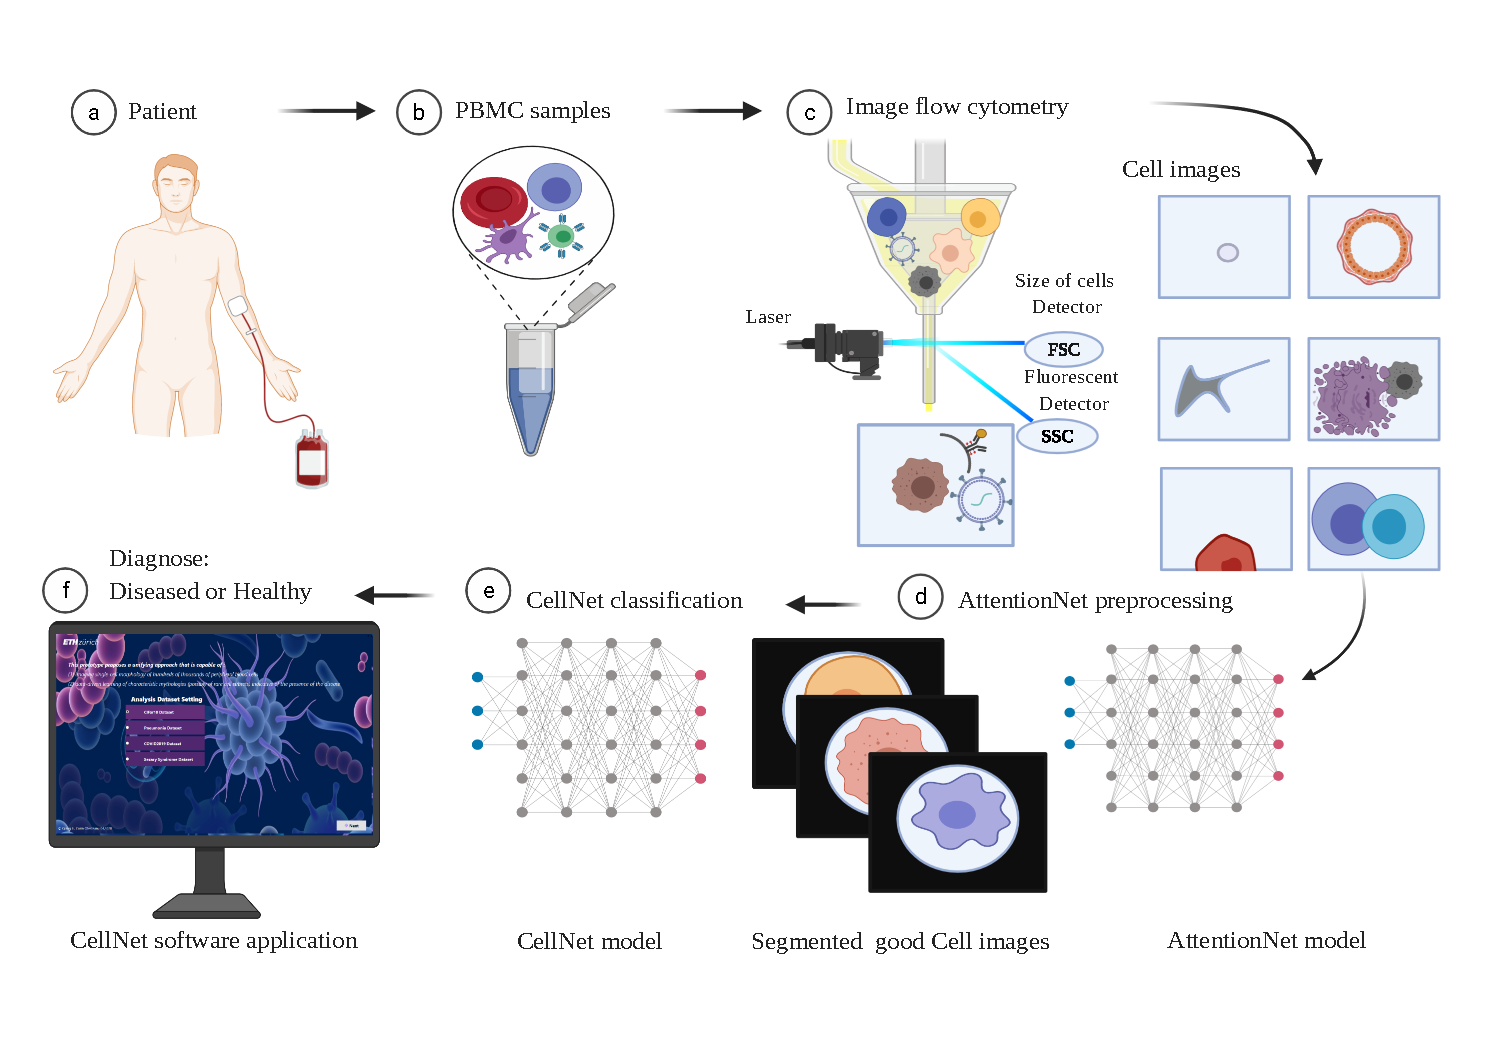
\includegraphics[width=\textwidth]{thesis-template-master/images/general workflow2.pdf}
	\label{fig:lenna}
	\end{center}
	\caption{General Workflow of Proposed Project. After Image Flow Cytometry (Morphological identification of tumor T-cells in the blood), those generated images can be categorized into 6 typical classes: lighting artifacts, out of focus cell, debris, contaminated cell, outside FOV cells  and multiple cell concatenated together. Using AttentionNet as a automatic detector and segment-or, we can filter out most of the artifacts in the images and only keep the morphological characteristics of the cell for CellNet classification. CellNet only has 8 novel Ghost module layers. CellNet software includes a total of 5 interfaces, 25 buttons, 10 user prompt functions and inherits 12 algorithms with the integration of 4 data sets.}
	\label{fig:lennas}
\end{figure}



In the first step, CellYolo approach has been developed to automatically annotate and segment cell types to single-cell images obtained from imaging flow cytometry experiments. These approach is based on deep learning paradigms that have emerged as a disruptive alternative to engineering-based techniques, which easily lead to a large amount of impure labelled data, and requires more resources and time. CellYolo as an efficient and accurate object detector emphasizing on small target, inherited the characteristics of the real-time detection of the YOLO network\cite{b33}, and at the same time avoided the low accuracy of the YOLO network in detecting small objects. Inspired from the YOLOv3-tiny network ,the K Means++ algorithm is an efficient approach of data pre-processing\cite{b18}. Experimental results demonstrate that CellYolo is not only a cost efficient solution for practical application( Labeling/Segmenting each image takes only 0.25 seconds in Intel CPU), but also an effective way of improving accuracy of object classification. We reproduced and integrated nearly 20 classic computer vision algorithms and test the performance with/without CellYolo preprocessing. With help of CellYolo preprocessing, the improvement based on state-of-the art algorithms in terms of Top-1 val-acc has been verified.

Once segmented, we proposed CellNet for Sezary Syndrom Cell / Healthy Cell classification. We applied similar Residual layer to forward and enable deeper neural network and follows the basic architecture of ResNet18 and GhostNet for its superiority \cite{b19}\cite{b20}. Replaced all the ResNet18 \cite{b20} point-wise convolutional layers (in total, 18 layers ) with Ghost Bottleneck \cite{b19}. In additional, we adopted the SE layers from Squeeze-and-Excitation Networks \cite{b24} to enhance useful features, scaling less inhibiting features map. In each ghost module, we first take pointwise conv to get a few intrinsic feature maps, then we utilized the linear cheap transformation such as depth-wise conv or affine transformation and wavelet transformation, as suggested by GhostNet\cite{b19}, here the depthwise conv was used.
Despite its simplicity (only 8 layers ghost module) and lower parameters(1/4 weights than ResNet18\cite{b20}, 1/2 weights than GhostNet\cite{b19}), CellNet establishes a new state-of-the-art on Sezary Syndrome Dataset (95.638\% Top-1 accuracy) and CIFar10 ( 90.051\% Top-1 accuracy)\cite{b21}. Moreover, the same method is also very competitive against recent leading Supervised approaches on Pneumonia Dataset (91.785\% Top -1 accuracy), where Inception V3 adopted after 7000 epochs reaches only 88.0\%\cite{b38}.

The remaining sections of this paper are organized as follows: Section 2 outlines some of the most relevant  prior work in medical image classification and segmentation including a short introduction about YOLOv3 \cite{b33} algorithm, the most important intuition of Residual learning, and recently invention of Ghost module.
Section 3 introduces our proposal. Section 4 presents experimental verification  and visualization on different benchmark dataset to validate the effectiveness of the proposed models and illustrates several ablative studies.Finally, conclusions are summarized in Section 5.

Our contributions. We proposes a unifying approach that is capable of (1) imaging single-cell morphology of thousands of peripheral blood cells and (2) data-driven learning of morphological characteristics, which are indicative of the presence of the disease.
Inspired by leading SOTA model, such as Deep Residual Learning\cite{b20} and Ghosts Net\cite{b19}, we proposed CellNet. Instead of stacking lots of point-wise convolutional layers and takes huge amount of convolutional manipulations, we can avoid the redundant feature maps by taking cheap operation. CellNet is originally designed for Sezary Syndrome Dataset and we provide comprehensive empirical evidence showing that CellNet has 1/4 weights than ResNet18 \cite{b20} and best classification performances on 
several other benchmarks such as CIFar10 \cite{b21} (92.451\% Top-1 accuracy), Pneumonia Dataset\cite{b38} (91.785\% Top-1 accuracy) and Sezary Syndrome Dataset (95.638\% Top-1 accuracy).
In addition, we purposed AttentionNet Network as an automated data pro-processing tool which provides a new intuition for object recognition, eliminating noise artifacts out of the image precisely can effectively improve the classification performance of many SOTA networks. Instead of manually labeling a large amount of data after Image flow cytometry and PBMC samples \cite{b12}, it is possible to automatically label an object with an accuracy of 88.64 \% in 0.25 seconds by using AttentionNet. 

We also produced the first COVID-19 Chest Xray/CT Dataset containing nearly 2,000 Xray/CT images (nearly 1,500 Healthy Xray/CT images and nearly 500 COVID-19 infected Xray/CT images). Experiments conducted on COVID-19 Datasets also demonstrated that the proposed CellNet is an impressive alternative of current baseline models, and our CellNet (94.719\% in Top-1 accuracy) outperforms the GhostNet\cite{b19} (92.739\%  in Top -1 accuracy) and other leading models. In addition, we developed a software application for potential diagnosis, which integrated with 12 leading SOTA models, including our CellNet. All code is available at \textit{https://github.com/Johnny-liqiang/CellNetUML}.



%3D data representations have been studied independently in their main field of application so far. In this thesis, however, we explore the potential of combining geodesic and Euclidean convolutions on point clouds and meshes simultaneously in the task of 3D semantic scene segmentation. In Figure 1.2, we illustrate our intuition that geodesic and Euclidean convolutions focus on different aspects of feature learning. Geodesic convolutions define proximity in terms of mesh neighbors reach￾able within  hops on the mesh. When applying convolutions on this neighborhood, we explicitly learn features focusing on the surface structure of the scene. For instance,in Figure 1.2a, the geodesic receptive field of the green center point just comprises vertices of the geodesically close chair surface. It therefore neglects geodesically remote but spatially close vertices of the table. Hence, we assume that geodesic convolutions are more likely to learn feature representations for object shapes.

%Contrastingly, Euclidean convolutions focus on the Euclidean proximity of vertices in terms of nn or radius neighborhoods in 3D space. They enable an information flow between geodesically disconnected parts of the scene and therefore, we assume that they learn the interaction between objects. For example, in Figure 1.2b, the convolution does not generate features only based on vertices of the chair but also based on the geodesically remote table. We assume that this contextual information helps to distinguish shape-wise similar classes such as chair and armchair. Concludingly, we pose the question if a combination of geodesic and Euclidean convolutions brings a significant benefit for the task of 3D scene segmentation. For this purpose, we have developed a simple yet effective multi-scale architecture called DualConvNet which combines Euclidean and geodesic convolutions in a parallel manner over multiple scales. Special provisions have been taken to guarantee the modularity of the architecture such that all effects are measurable in order to answer the research question in the ablation study experimentally.

%Our approach is mesh-centric in that sense that it consumes meshes as a half-edge data structure as well as defining (un-)pooling operations in terms of mesh simplification algorithms. This design decision is necessary to ensure a mesh structure in deeper network layers such that geodesic convolutions are well-defined. We therefore extend vertex clustering [RB93] and Quadric Error Metrics (QEM) [GH97] as two well-established algorithms from the geometry processing domain such that they can pool and unpool vertex sets from consecutive hierarchy levels. Pooling Trace Maps constitute this extension which comprises a look-up dictionary approach for obtaining pooled representatives in constant time. In order to make QEM pooling applicable for large-scale meshes, we finally present a novel sampling strategy for radius neighborhoods called Random Edge Sampling (RES) which outputs a sample set which guarantees an upper limit of a predefined expected sample size. In the ablation study, we take a closer look at the properties of RES.

%We empirically evaluate our proposed DualConvNet architecture on three publicly available benchmarks for 3D scene segmentation. We achieve competitive results on the ScanNet v2 [DCS+17], as well as the Stanford Large-Scale 3D Indoor Spaces Dataset (S3DIS) [ASZ+16]. Among graph convolutional approaches, we define a new stateof-the-art on both datasets. Moreover, on the recently published Matterport3D benchmark [CDF+17], we can report overall state-of-the-art results. We summarize the main contributions of this thesis as follows: 1 DualConvNet - our novel family of multiscale convolutional architectures - combines Euclidean and geodesic features for 3D semantic scene segmentation. 2 For creating mesh-centric multi-scale architectures, we extend two well-established mesh simplification algorithms as means of (un-)pooling operations. 3 Random Edge Sampling (RES) is a novel sampling method for sampling neighborhoods which guarantees an upper limit for the predefined expected size.
%Reducing the size of the neighborhood allows us to train networks with substantially fewer neighborhood sizes. However, we infer on test examples with larger sample sizes for better neighborhood approximations. 4 We conclude our work with a thorough ablation study which experimentally proves our claim that Euclidean and geodesic convolutions give a consistent benefit, independent of the pooling method and the notion of the neighborhood used in the architecture.



\chapter{Related Work}
\label{sec:examples}
This chapter will demonstrate some fun \LaTeX\ stuff.

\subsection[Awesome Figures in the TOC]{Awesome Figures} % (fold)

\label{sub:figures}
\begin{figure}[ht]
	\begin{center}
		\begin{subfigure}[b]{0.49\textwidth}
			\includegraphics[width=\textwidth]{thesis-template-master/images/lenna.png}
			\caption{Lenna}
			\label{fig:lenna}
		\end{subfigure}
		\begin{subfigure}[b]{0.49\textwidth}
			\reflectbox{\includegraphics[width=\textwidth]{thesis-template-master/images/lenna.png}}
			\caption{Lenna facing left}
			\label{fig:lenna_facing_left}
		\end{subfigure}
	\end{center}
	\caption{The famous Lenna image used in Computer Vision with subcaptions and a global caption.}
	\label{fig:lennas}
\end{figure}
The figure can be referenced in the text \eg\reffig{lennas}.
Also the subfigures can be referenced \eg\reffig{lenna}, \reffig{lenna_facing_left}.
% subsection figures (end)

\subsection{Citations} % (fold)
\label{sub:citations}
You can cite books from your bibliography \texttt{thesis.bib} (\eg \cite{cochrane}).
Abbreviations from \texttt{abbrev.bib} help in writing the entries.
% subsection citations (end)

\subsection{FixMe warnings}
\label{sub:fixme}
You can add warnings\fxwarning{WARNING} or notifications\fxnote{Note} to your text.
This will help you keep an overview on the places in the text you have to work on.

\section{Lorem}
\label{sec:lorem}
Lorem ipsum dolor sit amet, consectetur adipiscing elit. Pellentesque a nibh vulputate sapien condimentum vestibulum. Pellentesque tortor orci, aliquam eget odio a, aliquam tristique ante. Nulla tincidunt augue nec eros fringilla pretium. In ultrices fermentum erat quis imperdiet. Integer diam massa, egestas at nunc eu, aliquam placerat turpis. Suspendisse potenti. Nam luctus euismod nisl et volutpat. Sed at turpis ex. In facilisis quam neque, vitae lobortis felis fringilla quis. Phasellus porttitor leo eget massa efficitur, vel commodo diam venenatis. Vestibulum fringilla neque sed laoreet aliquam. Nulla sodales sodales velit ac fermentum.

In finibus pulvinar rhoncus. Mauris facilisis sit amet diam vel fermentum. Praesent laoreet dolor quis aliquet scelerisque. Integer condimentum, tortor dapibus vestibulum tristique, dui mauris posuere lectus, sed porttitor nisi dolor et ipsum. Nullam dignissim tortor ut mauris porta, ut gravida nisl fermentum. Morbi mattis egestas libero, quis elementum orci ornare nec. Morbi ultrices dolor eget arcu hendrerit ullamcorper. Nulla dui augue, molestie ac lobortis nec, pulvinar vitae quam. Cras neque nulla, pulvinar non vehicula quis, tincidunt id quam.

Etiam massa felis, tincidunt vel tincidunt ut, commodo id ipsum. Fusce blandit metus eget egestas mollis. Suspendisse interdum sem pellentesque ligula finibus, ac pretium metus lobortis. Integer id convallis felis, quis volutpat sapien. Phasellus elementum fermentum augue in mattis. Mauris pretium ipsum ornare augue sollicitudin hendrerit. Proin imperdiet interdum pretium. Nam in fringilla nisi, nec sollicitudin lacus. Pellentesque semper sapien vitae nulla scelerisque, ac convallis tortor porttitor. Fusce dolor tellus, porta vel magna vel, gravida ultrices eros. Integer sit amet nisl posuere, consectetur ante et, vulputate nulla. In a fringilla nisl.

Praesent vitae metus interdum, eleifend odio et, vehicula arcu. Suspendisse vulputate viverra enim ut convallis. Nunc nec gravida orci, suscipit interdum lacus. Morbi varius urna a dolor convallis, nec pulvinar massa maximus. Donec sed est ac odio scelerisque fringilla. Proin ac purus nec dolor porttitor tempor et sed dui. Vivamus arcu velit, vulputate sed fringilla dignissim, porta volutpat ipsum. Donec at venenatis lacus.

Vestibulum hendrerit, justo at laoreet dapibus, tortor orci placerat nunc, sed sodales massa quam eget dui. Pellentesque a ipsum non quam sodales pellentesque non eget sem. Pellentesque dignissim accumsan congue. Etiam nec odio at ipsum mollis lobortis. Nam tempus suscipit posuere. In mollis lacus in nulla lobortis sagittis id vitae lorem. Maecenas id libero sit amet lacus porta porta. Nam eu justo a enim efficitur commodo at et turpis. Vestibulum efficitur, elit eget vestibulum sollicitudin, ipsum massa luctus nunc, ut lobortis nisi magna ac velit. Morbi finibus elit a sagittis mattis. Duis ac scelerisque libero. Aliquam aliquam dui urna, quis pulvinar risus rutrum vitae. Curabitur quis lorem tristique, consequat magna vitae, tincidunt diam. Nam viverra velit nec leo mattis, eu mollis tellus imperdiet. Vestibulum nibh nulla, porta eget venenatis non, commodo pulvinar ex.
% section lorem (end)

\section{Ipsum}
\label{sec:ipsum}
Mauris ultrices commodo risus, mollis congue dui scelerisque elementum. Nam ac dictum augue. Vestibulum convallis vel dui et porttitor. Aenean a commodo justo. Integer condimentum pulvinar massa, eu venenatis metus bibendum aliquam. Aenean ac tristique nisl, ut maximus tortor. Duis venenatis ultricies tellus, non dignissim metus feugiat vel. Curabitur a lorem ligula. Nunc commodo erat id mauris condimentum euismod. Etiam vel sodales augue. Donec id tincidunt tellus. Pellentesque tempus ultricies lobortis. Vestibulum magna velit, iaculis rhoncus aliquet sed, congue vitae risus. Suspendisse iaculis, nibh at imperdiet tincidunt, mi metus pharetra tortor, quis posuere est ante id ex.

\subsection{Dolor sit} % (fold)
\label{sub:dolor_sit}
Fusce a tortor sit amet quam suscipit commodo non eget massa. Vestibulum semper accumsan tristique. Aenean posuere laoreet sollicitudin. Vivamus nec ligula et nunc ornare pellentesque. Aenean vulputate vestibulum risus facilisis condimentum. Morbi ac ex magna. In feugiat ligula in nisi tincidunt malesuada. Morbi convallis nunc id nisi ultrices venenatis. Donec in felis vel lectus lobortis malesuada. Morbi ut neque nulla. Quisque augue nibh, tempor in elit at, convallis gravida enim. Integer iaculis nibh eget commodo mollis. Vivamus at viverra eros. Pellentesque eu elit velit. Nunc nec ligula diam.

Suspendisse tempus id neque vel ultricies. Vivamus efficitur dui non enim vehicula, sed faucibus massa consectetur. Aenean lacinia sapien quis pellentesque auctor. Vestibulum auctor dui a orci imperdiet, vitae posuere sapien vulputate. In eget augue quis erat rhoncus dignissim ut nec felis. Ut dignissim, ligula a porta sollicitudin, erat enim maximus sapien, vitae vehicula ligula eros sed mauris. Maecenas vehicula, mauris nec sagittis pellentesque, mauris turpis volutpat sapien, vitae mattis magna enim sit amet ligula.

Duis sem elit, egestas eleifend auctor quis, elementum nec nisi. Sed sed ipsum ac mi rutrum pretium. Maecenas a pulvinar eros. Integer eget pretium arcu, at egestas ante. Donec neque magna, pellentesque in justo et, convallis congue enim. Etiam et quam sit amet mi ullamcorper pretium vitae id ligula. Maecenas ac ligula justo. Curabitur gravida nunc tincidunt auctor rhoncus. Donec sit amet ante ipsum. In quis ullamcorper ex. Cras ac ullamcorper orci, et aliquet enim. Nam in elit sit amet tortor finibus interdum.

Sed ac facilisis augue. Cras nec nisl consequat, gravida tortor vitae, tincidunt nisi. Duis posuere eu orci at luctus. Morbi nec malesuada arcu. Aliquam erat volutpat. Maecenas pharetra in nisi sed molestie. Cras id urna eu nunc ullamcorper volutpat a sit amet elit. Donec tincidunt laoreet ipsum, a sagittis tellus laoreet sodales. Aliquam in ultricies sapien, semper tempus nisl. Pellentesque lectus nisi, tempus ut fermentum quis, pulvinar ac velit.

Duis laoreet pellentesque libero, egestas mattis ante maximus id. Donec convallis felis vel neque placerat ornare. Curabitur id iaculis lectus. Duis vitae tristique lectus. Sed maximus aliquet nisl, quis bibendum sem. Vestibulum ut ipsum a risus fermentum dapibus tincidunt semper lorem. Proin ante ante, euismod sed turpis eu, dictum bibendum ipsum. Praesent fermentum volutpat metus, quis fringilla arcu fermentum eget. Suspendisse quis condimentum sapien, ut sollicitudin metus. Ut in volutpat enim. Phasellus sapien est, varius in condimentum et, auctor et augue. Donec mattis malesuada leo, vitae pellentesque metus ornare vel. Pellentesque massa nulla, aliquet nec metus et, auctor porta lacus. Fusce ac ex faucibus, placerat nibh ac, fermentum leo. Curabitur interdum fermentum lacus, quis mollis erat suscipit nec. Vestibulum vel pellentesque ipsum, sit amet ultrices quam.

Proin vestibulum nec risus ut porttitor. Pellentesque porta ipsum elit, quis lacinia quam vehicula eu. Nulla consectetur nulla ac euismod tincidunt. Curabitur quis auctor neque, eget viverra nibh. Vivamus porttitor aliquam leo id iaculis. Cras sed dapibus quam. Mauris ullamcorper lacus ut porta sollicitudin. Proin accumsan finibus dolor, eu suscipit massa interdum non. Maecenas lobortis sit amet leo in fringilla.
% subsection dolor_sit (end)

\subsection{Amet} % (fold)
\label{sub:amet}
Nulla nec accumsan risus. Mauris consectetur ex vel tempus posuere. Quisque sit amet placerat risus, vitae suscipit massa. Maecenas molestie scelerisque ipsum, ac porta purus dapibus ut. Phasellus rhoncus sit amet lorem nec vulputate. Sed quis erat erat. In congue at nisi in tristique. Pellentesque auctor, nunc ut hendrerit laoreet, neque urna sagittis orci, sit amet accumsan nisi velit et diam. Phasellus sit amet posuere mauris. In hac habitasse platea dictumst. Quisque eget consectetur lectus. Nam finibus porttitor augue, sed fermentum augue vehicula id. Pellentesque convallis auctor condimentum. Donec at pharetra ipsum, id consequat turpis.

Interdum et malesuada fames ac ante ipsum primis in faucibus. Ut semper urna ac imperdiet imperdiet. Duis aliquam enim vel dolor euismod, vel posuere enim cursus. Sed tristique dui vitae lacus facilisis gravida. Donec quis nisl sed mi iaculis placerat. Integer dictum elit quis enim venenatis, eu egestas odio porttitor. Proin ac ipsum semper, tincidunt lectus vitae, elementum nibh. Nunc facilisis scelerisque nibh, eget tincidunt tellus rhoncus non. Etiam luctus tellus a eros dignissim, nec mollis lacus elementum. Fusce tincidunt porta efficitur. Aenean id volutpat sapien, vel fermentum augue. Cras sed dapibus risus. Etiam mi felis, blandit sed rutrum ut, rhoncus sit amet nisi. In quis sem finibus, posuere tortor sit amet, lacinia enim. Proin nibh neque, commodo luctus sagittis in, luctus non diam. Donec semper commodo nunc, et laoreet risus feugiat eget.

Phasellus pulvinar tellus id libero mattis, quis sollicitudin arcu hendrerit. Quisque nec posuere mi, nec luctus magna. Ut consectetur ante vel velit congue, ac vulputate turpis molestie. Maecenas quis diam dolor. Pellentesque rhoncus porta condimentum. Aliquam malesuada leo quis placerat posuere. Duis maximus mauris hendrerit lacus viverra auctor. Morbi in urna libero. Donec dictum, justo a tincidunt dictum, enim mauris condimentum erat, non lobortis ex risus sed sapien. Sed ac sapien luctus, vehicula justo lobortis, congue orci. Praesent ultricies turpis vel ex pretium placerat.

Maecenas ultricies dolor eget lorem vestibulum sodales. Nam tortor elit, bibendum malesuada ante et, pharetra mollis tellus. Cum sociis natoque penatibus et magnis dis parturient montes, nascetur ridiculus mus. Duis ligula nisi, blandit eget condimentum ut, facilisis et urna. Nunc sed velit a urna mattis malesuada. Etiam convallis quam libero, quis maximus metus lacinia non. Donec cursus, justo feugiat scelerisque pretium, leo felis lacinia nulla, vel pharetra mi sem id risus. Aliquam eu metus ac dolor varius ultrices. Nulla faucibus lorem sit amet libero aliquam ullamcorper. Nulla eu quam vulputate, volutpat sapien in, tincidunt neque. Nullam sapien erat, iaculis sed orci vel, porta efficitur lorem. Phasellus a nibh sagittis, iaculis erat ut, egestas risus. Nulla diam massa, dictum at vehicula quis, malesuada sed mi. Morbi vitae dolor quam. Ut bibendum rutrum felis, quis dignissim felis interdum nec.

In vitae faucibus erat, at tristique nisi. Mauris eget sodales lacus, eget mattis ipsum. Integer at iaculis purus. Quisque non elementum orci. Nulla non orci convallis, convallis orci et, rhoncus felis. Fusce nec velit enim. Nam imperdiet et sem vitae gravida. Cum sociis natoque penatibus et magnis dis parturient montes, nascetur ridiculus mus. Mauris placerat maximus aliquet. Donec sagittis augue rutrum consequat egestas.

Vestibulum faucibus, ante tincidunt porttitor malesuada, arcu eros mollis elit, id gravida ante mauris in nisl. Morbi eros sem, ultrices vel leo a, efficitur scelerisque mi. Sed posuere sit amet erat quis facilisis. Vivamus posuere sem ut orci sodales aliquam. Nulla facilisi. Etiam pulvinar finibus augue, vel interdum purus placerat sit amet. Morbi placerat interdum aliquet. Nulla fermentum urna at hendrerit tempus. Vestibulum vitae ultrices dolor.

Duis fringilla mauris ut efficitur egestas. Praesent quis sapien risus. Nulla quis quam nec nulla semper viverra quis vel lorem. Donec commodo faucibus magna eget vestibulum. In hac habitasse platea dictumst. Fusce ullamcorper odio nulla, nec egestas enim efficitur et. Donec pharetra ipsum libero, nec mollis quam posuere nec. Aliquam vitae egestas arcu. Quisque interdum rutrum neque convallis convallis. Nulla non consequat quam. Pellentesque et nisi dictum, posuere nibh vel, eleifend turpis. Praesent tincidunt sodales leo ac efficitur. Phasellus arcu ipsum, molestie ac orci vitae, euismod sodales metus.

Duis est lectus, vestibulum at arcu sed, suscipit pellentesque nisi. Nulla arcu ante, feugiat nec diam ac, auctor ullamcorper nibh. Praesent a arcu sed massa vestibulum condimentum. Etiam gravida at massa in ullamcorper. Aenean finibus, metus et consectetur viverra, augue eros finibus purus, eget sollicitudin erat purus feugiat sapien. Morbi mattis orci sit amet sem semper, non fringilla quam dignissim. Fusce aliquam dolor et lectus pellentesque lobortis. 
% subsection amet (end)
% section ipsum (end)
% section examples (end)





























\chapter{Methodology}
\label{sec:Methodology}
The purpose of this thesis is to invent a unifying approach that is capable of not only imaging single-cell morphology of thousands of peripheral blood cells, but also data-driven learning of characteristic mythologies indicative of the presence of the disease. With this in mind, we introduce a novel family of deep hierarchical network architectures called AttentionNet. Its goal is to leverage a simple but well-established architecture for nearly-semantic segmentation in order to ensure 
higher precision classification task. Thus, we are able to base our claims about multi-Scale prediction framework and multiple layers concatenation of original YOLOv3 architecture on a variety of experiments individually (see Chapter 5). The idea of this novel AttentionNet architecture is to combine lighter-weight layers  and k-means++ techniques in pre-processing, and GBCIOU multi-object segment techniques such that the network explores and archives the nearly-semantic segmentation for cells with lower cost computation cost and complexity.

For biomedical images processing, due to different experimental conditions, such as lighting condition and various  experimental objects, noise deviations are likely to appear on the sampled cell images\cite{b6}\cite{b7}, those noise and variability in the background would be confounding variables.
When applying attentionnet first, we explicitly learn features focusing on the morphology structure of the object. As we originally designed the unifying approach for Sezary Syndrome, which is an aggressive cutaneous T cell lymphoma that is characterized by presence of tumor T cells with abnormal nucleus morphology in the peripheral blood. Morphological identification of tumor T cells in the blood is currently still the gold standard.
Hence, we assume that after AttentionNet segmentation convolutions are more likely to learn feature representations only for cell objects as only the cell objects are preserved.

Modern architectures leverage multi-scale hierarchies in order to learn feature representations at different resolutions from fine-grained, highly localized features to coarse but semantically enriched features, such as original YOLO network and other state-of-the-art models. On the other hand, it also increases  the complexity of network, requires excessive computational cost and has insufficient sensitivity to customer datasets.

AttentionNet however discards Darknet feature extraction layer of original YOLO, which is a multi convolutional stacked layer, and relies on two yolo output layers. Because the prior of the predicted box is known upfront by k-Mean++ clustering we introduced. Thus, only a few up-sampling layers additional are needed to give a satisfied accurate prediction of the cell position. then, circle detection algorithm will convert Square bounding box to nearly semantic cell prediction while guaranteeing user-defined quality requirements of the cell structure.

Since NMS(Non-Maximum Suppression) of YOLOV3 will only removing prediction boundary boxes that have a high overlap and a low class score, we cannot guarantee good performance in cases such as:multiple cells overlap each other and have high objectiveness scores, or multiple cells do not overlap but are presented in the same frame. It is inevitable to utilize GBCIOU to eliminate objects with relative lower objectiveness score while maximizing retention of overlapping cells.

It is worth noting that the AttentionNet is not involved in the task of cell classification. We therefore introduce CellNet. The main novelty of CellNet is that it creatively combines the features of ResNet\cite{b20} that are easy to expand, easy to understand, and extremely high classification accuracy, and the feature of GhostNet\cite{b19} module that uses a small amount of linear cheap operation to reduce  redundant feature maps, thereby achieving a lighter weight, real-time processing and higher classification accuracy network, especially suitable for the use of complex medical data sets.
%is currently still the gold standard\cite{b3}. There are huge amount of cell images produced from image flow cytometry process, including both healthy data set and diseases data set for comparison. 


\section{AttentionNet}
\label{sec:lorem}




\subsection{Network Architecture} % (fold)
\label{sub:citations}

In Table 3.1, we present our multi-scale AttentionNet architecture which adopts the YOLOV3-Tiny architecture as its fundamental building block in order to process more efficiently on small target. We follow the same
symmetrical encoder-decoder architecture with additional skip-connections interconnected them in the same hierarchy level. At each hierarchy level, we perform several point-wise convolutions in a consecutive manner. 

\begin{table}[h]
\centering

\scalebox{0.90}{
\begin{tabular}{@{}clllll@{}}
\toprule
\multicolumn{1}{l}{\textbf{layer}} & \textbf{Type}                & \multicolumn{1}{l}{\textbf{Filters}} & \textbf{Size/Stride} & \textbf{Input}       & \textbf{Output}                          \\ \midrule
0                                  & Convolutional                & 16                                   & $3\times3$/1       & 416\times416\times3            & 416\times416\times16                               \\
1                                  & Maxpool                      &                                      & $2\times2$/2                & 416\times416\times16           & 208\times208\times16                               \\
2                                  & Convolutional                & 32                                   & $3\times3$/1                & 208\times208\times16           & 208\times208\times32                               \\
3                                  & Maxpool                      &                                      & $2\times2$/2                & 208\times208\times32           & 104\times104\times32                               \\
4                                  & Convolutional                & 64                                   & $3\times3$/1                & 104\times104\times32           & 104\times104\times64                               \\
5                                  & Maxpool                      &                                      & $2\times2$/2                & 104\times104\times64           & 52\times52\times64                                 \\
6                                  & Convolutional                & 128                                  & $3\times3$/1                & 52\times52\times64             & 52\times52\times128                                \\
7                                  & Maxpool                      &                                      & $2\times2$/2                & 52\times52\times128            & 26\times26\times128                                \\
8                                  & Convolutional                & 256                                  & $3\times3$/1                & 26\times26\times128            & 26\times26\times256                                \\
9                                  & Maxpool                      &                                      & $2\times2$/2                & 26\times26\times256            & 13\times13\times256                                \\
10                                 & Convolutional                & 512                                  & $3\times3$/1                & 13\times13\times256            & 13\times13\times512                                \\
11                                 & Maxpool                      &                                      & $2\times2$/1                & 13\times13\times512            & 13\times13\times512                                \\
12                                 & Convolutional                & 1024                                 & $3\times3$/1                & 13\times13\times512            & 13\times13\times1024                               \\
13                                 & Convolutional                & 256                                  & $1\times1$/1                & 13\times13\times1024           & 13\times13\times256                                \\
14                                 & Convolutional                & 512                                  & $3\times3$/1                & 13\times13\times256            & 13\times13\times512                                \\
15                                 & Convolutional                & {\color[HTML]{CB0000} \textbf{18}}   & $1\times1$/1                & 13\times13\times512            & {\color[HTML]{CB0000} \textbf{$13\times13\times18$}} \\
16                                 & YOLO                         &                                      &                      &                      &                                          \\
17                                 & \textbf{Rout13}              &                                      &                      &                      &                                          \\
18                                 & Convolutional                & 128                                  & $1\times1$/1                & 13\times13\times256            & 13\times13\times128                                \\
19                                 & Upsampling                   &                                      & $2\times2$/2                & 13\times13\times256            & 26\times26\times128                                \\
20                                 & \textbf{Route 19, 8}         &                                      &                      &                      &                                          \\
21                                 & Convolutional                & 256                                  & $3\times3$/1                & 26\times26\times384            & 26\times26\times256                                \\
22                                 & Convolutional                & {\color[HTML]{CB0000} \textbf{18}}   & $1\times1$/1                & 26\times26\times256            & {\color[HTML]{CB0000} \textbf{$26\times26\times18$}} \\
23                                 & YOLO                         &                                      &                      &                      &                                          \\ \bottomrule

\end{tabular}}
\caption{\textbf{AttentionNet network structure}. Final YOLO Output should equal to $3\times(classes+5))$}
\end{table}

The attributes of self-detection and labeling, of nearly real-time resolve and of general resource requirements mainly characterize the AttentionNet Network. At the beginning it is  similar to YOLOv3\cite{b33} that the input image is divided into an $M \times M$ grid. Then $B$ bounding boxes and confidence score are defined in each grid cell. Each grid cell predicts $C$ conditional probabilities, denoted as $P(Class_{i}\mid Object_{j})$ for $i$ classes and object $j$. If there is an object $j$ in the grid, then indicated the objectiveness score $P(Object_{j})$  equal to $1$\cite{b18}. Here, we refer the initiatives from YoloV3, the confidence score also represents the accuracy of the box prediction, which is defined as $GIOU_{Ground truth}^{Predition}$. Unlike the originally YOLOv3\cite{b33}, instead of using Intersection‐Over‐Union (IOU), we use $GIOU$ with higher precision, which refers to the generalized intersection area between the predicted bounding box and ground truth box.

It should be noted that each grid cell predicted conditional class probability is not same as the confidence score. These often leads to misunderstanding of the fact that the former $P(Class_{i} \mid Object_{j})$ is predicted in each grid, while the $P(Object_{j}) \times GIOU_{Ground truth}^{Predition}$ is predicted in each bounding box\cite{b18}. 
Finally Class Score $S$ is defined as follow (1): \label{eq}

\begin{equation}
\begin{split}
$S&=P(Class_{i}\mid Object_{j}) \times P(Object_{j}) \times GIOU_{Ground truth}^{Predition} \\
$& = P(Class_{i}) \times GIOU_{Ground truth}^{Predition} $\label{eq}
\end{split}
\end{equation}

The Class Score $S$ computed the probability of the object $j \in  i$ class appearing in the box, as well as how well the bounding box fits each object $j$.






\subsection{Multi Scale Tensor Prediction Framework}
\label{sub:fixme}

The original YOLOv3\cite{b33} used the darknet front-end feature extraction module, but the detection performance on Sezary Syndrom dataset is unsatisfied. On the contrary, AttentionNet with only $13 \times 13$, $26 \times 26$ yolo scale output tensors adopts multi-scale fusion, and K means++ clustering\cite{b18} techniques, outperforms TF-Yolo\cite{b18} and  YOLOv3 \cite{b33}, which has $13 \times 13$, $26 \times 26$, $52 \times 52$ yolo scale output tensor. In order to train a suitable segment-or, it is recommended to choose corresponding scale tensors refer to different data sets. 

We use a YOLOV3 like architecture due to its modularisation capabilities. In the ablation study, we individually measure the impact of all architectural components. Here, we vary the tensor Multi Scale Tensor, as well as the number of hierarchy levels used by the architecture. Moreover, we vary the number of point-wise convolution layers to measure the effect of each Yolo tensor output independently and in parallel. Hence, we make reasonable
claims about the combination of only $13 \times 13$, $26 \times 26$ yolo scale output tensors.

\begin{figure}[h]
	\begin{center}
		\begin{subfigure}[b]{0.49\textwidth}
			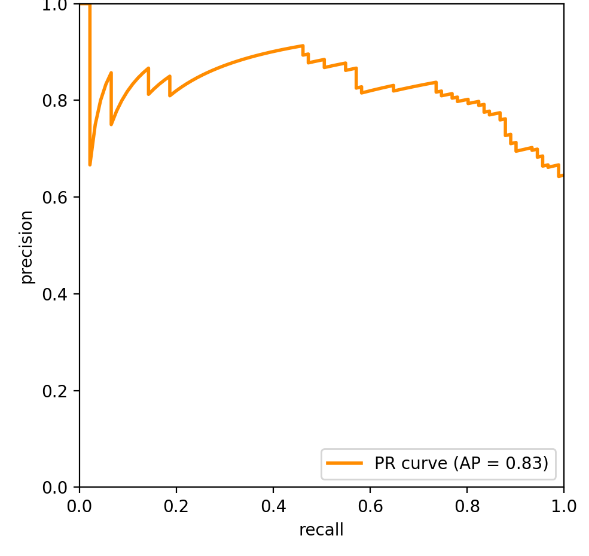
\includegraphics[width=\textwidth]{thesis-template-master/images/2 tensor cellyolo PR on val dataset.png}
			\caption{$13 \times 13$, $26 \times 26$ tensor Cellyolo PR on val dataset}
			\label{fig:res18}
		\end{subfigure}
		\begin{subfigure}[b]{0.49\textwidth}
		    \centering
			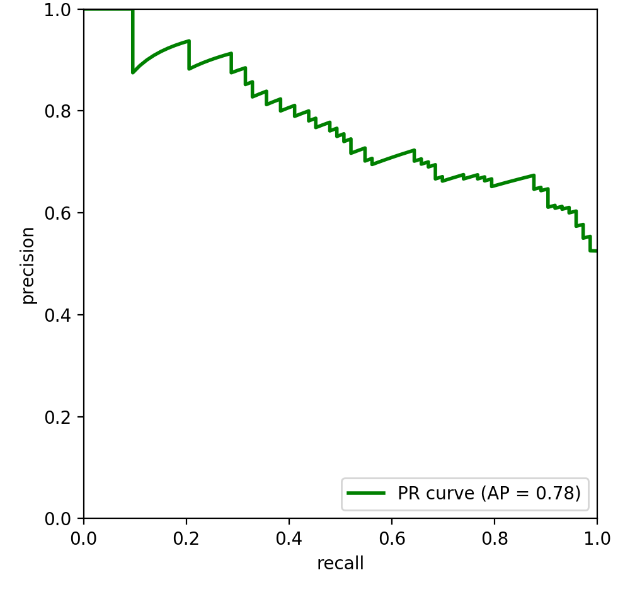
\includegraphics[width=\textwidth]{thesis-template-master/images/52 tensor cellyolo PR on val dataset.png}
			\caption{$52 \times 52$, $26 \times 26$tensor Cellyolo PR on val dataset}
			\label{fig:cellnet}
		\end{subfigure}
	\end{center}
	\caption{Precision-Recall curve on val sub-dataset of Sezary Syndrom dataset (1k training image, 726 test image), in terms of different scale yolo output layers}
\end{figure}



\subsection{K‐means++ Clustering in Pre-processing}
K‐means++ clustering is an approach commonly used to adaptive partition a dataset into groups. It is necessary to specify the number of cluster centers in advance. The k‐means++ algorithm generally uses the Euclidean distance to measure the distance between two points. Instead of using prior 9 box given by YOLOv3 trained on COCO dataset, for our customer dataset, it's noteworthy that give the prior knowledge of ground truth box. Using small subset of manually annotated cell, we can improve $GIOU$(ground truth box position, prediction box location) scores, and these will leads to better class scores as well and in final achieve higher accuracy.

\begin{figure}[h]
	\begin{center}
		\begin{subfigure}[b]{0.49\textwidth}
			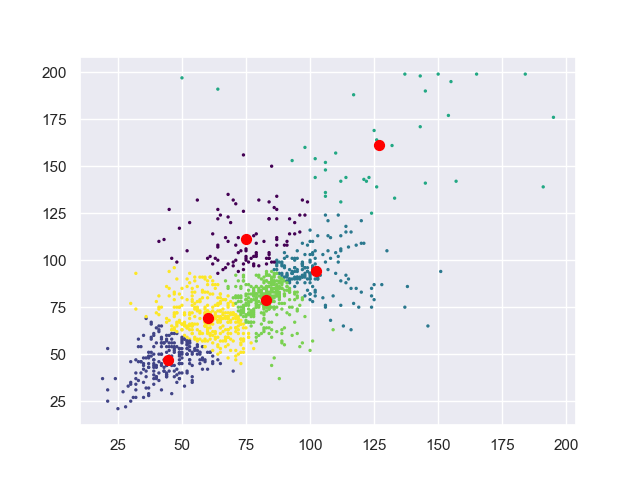
\includegraphics[width=\textwidth]{thesis-template-master/images/Figurefor 1480_1.png}
			\caption{ Six prior boxs}
			\label{fig:res18}
		\end{subfigure}
		\begin{subfigure}[b]{0.49\textwidth}
		    \centering
			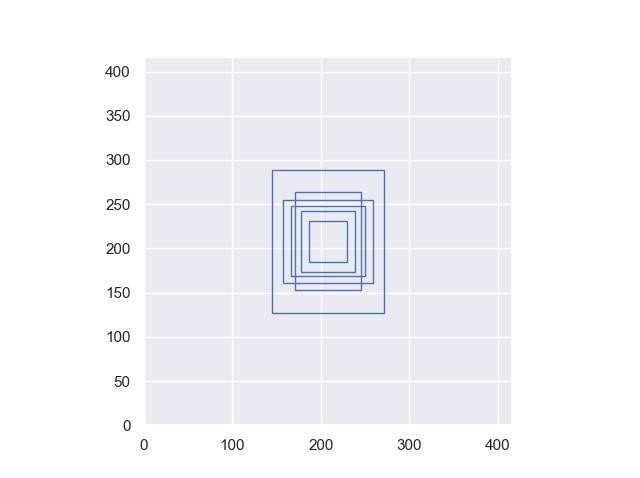
\includegraphics[width=\textwidth]{thesis-template-master/images/Figure_for1480.png}
			\caption{The cluster distribution}
			\label{fig:cellnet}
		\end{subfigure}
		\begin{subfigure}[b]{0.49\textwidth}
			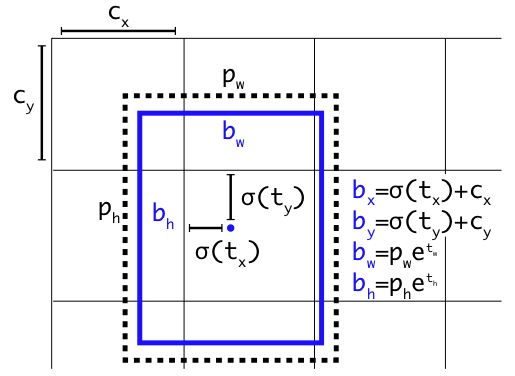
\includegraphics[width=\textwidth]{thesis-template-master/images/anchor.JPG}
			\caption{ Prior box and location prediction box}
			\label{fig:res18}
		\end{subfigure}
	\end{center}
	\caption{\textbf{The comparison between normal convolutional layer in \cite{b26}\cite{b27}\cite{b28} and ghost module}. We only take point-wise convolution once to get a few intrinsic feature maps, then we utilized the linear cheap transformation to generate ghost map with lower cost.}
\end{figure}

Nevertheless, there are the following three scale targets in the dataset: large‐scale targets, moderate‐scale targets, and small‐scale targets [30]. The main steps of the K‐means++ method are as follows:   

Step 1: Choose an initial center t1 uniformly at random from the dataset X.

Step 2: Choose the next center ti , selecting  with probability
where D(x) is the distance from a data point x to the closest center.

Step 3: Repeat Step 2, until D x( ) is the shortest distance. After which, k center is chosen.

Step 4: Define center 

Step 5: For i , set the cluster Ti to be the set of points in X that are closer to
ti than they are to tj for all j i.

Step 6: For i k , set ti to be the center of mass of all points inTi

Step 7: Repeat Step 5 and Step 6 until T converges.

The definition of the three sizes of targets here refers to the proportion that they are in the entire image.

\begin{figure}[h]
	\begin{center}
		\begin{subfigure}[b]{0.49\textwidth}
		    \centering
			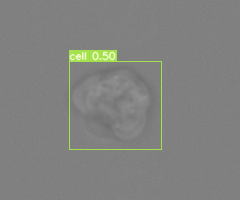
\includegraphics[width=0.9\textwidth]{thesis-template-master/images/withkmean.png}
			\caption{With k-means++ cluster}
			\label{fig:cellnet}
		\end{subfigure}
		\begin{subfigure}[b]{0.49\textwidth}
		    \centering
			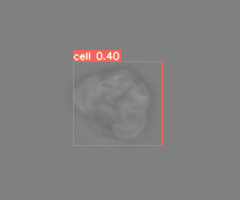
\includegraphics[width=0.9\textwidth]{thesis-template-master/images/withoutkmean.png}
			\caption{Without k-means++ cluster}
			\label{fig:cellnet}
		\end{subfigure}
		\begin{subfigure}[b]{0.49\textwidth}
		    \centering
			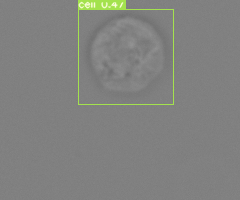
\includegraphics[width=0.9\textwidth]{thesis-template-master/images/withkmean1.png}
			\caption{With k-means++ cluster}
			\label{fig:cellnet}
		\end{subfigure}
		\begin{subfigure}[b]{0.49\textwidth}
		    \centering
			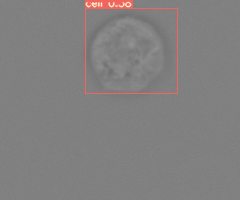
\includegraphics[width=0.9\textwidth]{thesis-template-master/images/withoutkmean2.png}
			\caption{Without k-means++ cluster}
			\label{fig:cellnet}
		\end{subfigure}
	\end{center}
	\caption{\textbf{The comparison between normal convolutional layer in \cite{b26}\cite{b27}\cite{b28} and ghost module}. We only take point-wise convolution once to get a few intrinsic feature maps, then we utilized the linear cheap transformation to generate ghost map with lower cost.}
\end{figure}

As mentioned above, YOLOv3 algorithm has achieved end‐to‐end training and high‐speed target detection. However, some problems still exist. Conventional YOLO divides each image into a fixed grid, which results in the number of detected objects will be limited. The fixed parameters provided by anchor are suitable for the targets in the VOC datasets, while they are not adapted to the targets in specific scenes. Common targets, such as vehicles, tanks, and airplanes, have a large aspect ratio. Therefore, this section takes advantage of the ideas in Fast R‐CNN and SSD to re‐cluster according to a spacific scenario. In the beginning, the network manually sets a priori box. To guarantees the selection of network is more subjective, and it would make the deep network easier to learn. Furthermore, its predictions perform better than the original method. In order to optimize the adapted parameters and select appropriate anchor box size, the designed network needs to recluster according to real application domains. In this way, the AttentionNet network achieve nearly semantic prediction, meanwhile, it is insensitive to small objects particularly.




\subsection{Loss function} % (fold)
\label{sub:citations}

Contrarily to the original implementation of YOLOv3 (Chapter 2.3.2), we calculate the loss function by means of three parts. Here, we divide them into three compositions, the loss between the ground truth box and the prediction box, the confidence score loss, the final cross entropy loss for class label. First part is the prediction bounding box loss, second part indicates the confidence loss and final part represents the class label loss. k means the classes, the conf states the confidence, and the 10647 generated from 2535 prediction bounding boxes. It is equal to $(13\times13\time3+26\time26\time3)=2535$ in contrast to originally YOLOv3 has $(13\times13\time3+26\time26\time3+26\time26\time3)=10647$ prediction bounding boxes.

\begin{equation}
\begin{split}
$Loss&=\frac{1}{2}\sum_{i=1}^{2535}\lambda _{obj}\times \{ \left ( 2-truth_{w} \times truth_{h}\right )\times  \sum_{r\in \left ( x,y,w,h \right )}^{}\left ( truth_{r}-predict_{r} \right )^{2} \\$
$&+ \sum_{k-1}^{r=0} \left ( \left ( r==truth_{class} \right )-predict_{class_{r}} \right )^{2}  \} + \left ( truth _{conf}-predict_{conf}\right )^{2}$  \label{eq}
\end{split}
\caption{\textbf{Loss function adopted in AttentionNet}.}
\end{equation}


\textbf{ The Loss for Bounding Box}:
\begin{equation}
\begin{split}
$\lambda _{obj}\times \left  \left ( 2-truth_{w} \times truth_{h}\right )\times \sum_{r\in \left ( x,y,w,h \right )}^{}\left ( truth_{r}-predict_{r} \right )^{2}$ \label{eq}
\end{split}
\caption{\textbf{The Loss for Bounding Box}.}
\end{equation}
In YOLOv1, the author did find the square root of the width and height (w, h), in order to Weakening the influence of the bounding box size on the loss value. Here, we are following YOLOv3 priority suggestions do not adopt the square root method, but added a weight related to the size of the  object box size. namely with weight = $  2-truth_{w} \times truth_{h}  $, value range from (1~2). In contrast to the first version of YOLO network, which adopted the IOU loss to calculate the loss between  prediction box and prior, the YOLOv3 imporved the accuracy by 1\% under the  contribution of GIOU loss. 

In cvpr2019 paper GIOU, they proposed a new way to optimize boundary boxes mode, defined as generalized IOU, the bounding box is generally composed of the upper left and lower right corners of the coordinates, denoted as (x, y, x2, y2). Note that this is actually a vector, and vector distances are generally can be measured by either the L1 norm or the L2 norm.

However, when either the L1 or L2 norms is the same, it was found that the values of both IOU and GIOU are very different, indicating that the use of the L paradigm to measure the the distance between  the prediction and the real ground truth is inappropriate.



\begin{figure}[h]
	\begin{center}
		\begin{subfigure}[b]{0.49\textwidth}
		    \centering
			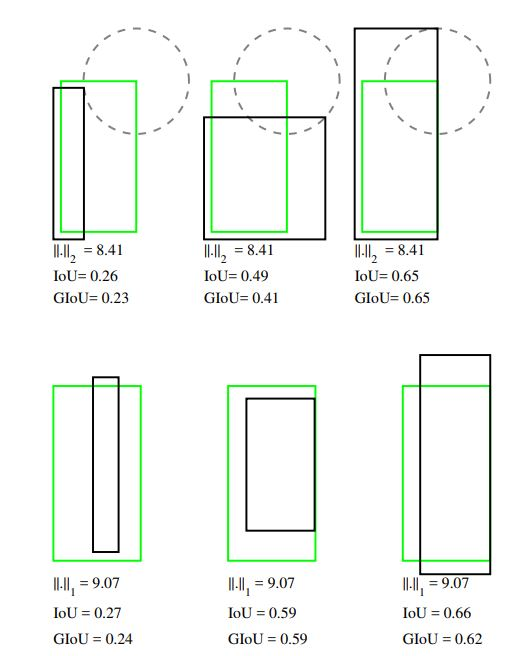
\includegraphics[width=0.9\textwidth]{thesis-template-master/images/l2loss.JPG}
			\label{fig:cellnet}
		\end{subfigure}
	\end{center}
	\caption{Two sets of examples with the bounding
boxes represented by two corners (x1, y1, x2, y2) for first row, center and size (xc, yc, w, h) for second row. For all three cases in each set$ ℓ2$
norm distance, and  $ℓ1$-norm distance, between the representation of two rectangles are exactly same value, but their IoU and GIoU values are very different.}
\end{figure}


In this case, the IOU is commonly used in academia to measure the similarity between two boundaries, but we found experimentally that there are two obvious drawbacks to using IOU which makes it less suitable for the loss function.

First, when there is no overlap between the prediction box and the ground truth. An IOU value of 0 results in a gradient of 0 when optimizing the loss function, meaning that optimization is not possible.

secondly, even if the prediction box and the real box overlap and have the same IOU value, the detection effect will be very different. This is indistinguishable by IOU, because IOU is the same, but this can be reflected by GIOU . If the two bounding boxes overlap the better, the better the alignment, the higher the GIOU value.

\textbf{ The confidence score loss}:
\begin{equation}
\begin{split}
$\left ( truth _{conf}-predict_{conf}\right )^{2}$ \label{eq}
\end{split}
\caption{\textbf{The Loss for Bounding Box}.}
\end{equation}


First, we should find the prediction bounding box with the largest IOU value of the real ground truth. If the largest IOU is less than the threshold, then the prediction is considered to contain no objects, and it is the background grid. Then we calculate the   confidence loss (we hope that if the grid contains objects, then the confidence of the prediction box output is 1, and 0 when there is no object). The confidence $\lambda _{obj}$ comes from focal loss. It indicates the confidence level to determine if there is an object in the grid.

\textbf{ The cross entropy loss for class label:}
\begin{equation}
\begin{split}
$\lambda _{obj}\times \sum_{k-1}^{r=0}  ( ( r==truth_{class}  )-predict_{class_{r}} )^{2} $ \label{eq}
\end{split}
\caption{\textbf{The Loss for Bounding Box}.}
\end{equation}
Finally,we  utilize the cross entropy loss to generate the class label.


\subsection{GBCIOU and Circle segmentation}
\label{sub:fixme}
You can add warnings\fxwarning{WARNING} or notifications\fxnote{Note} to your text.
This will help you keep an overview on the places in the text you have to work on.





\section{CellNet}
\label{sec:ipsum}
Mauris ultrices commodo risus, mollis congue dui scelerisque elementum. Nam ac dictum augue. Vestibulum convallis vel dui et porttitor. Aenean a commodo justo. Integer condimentum pulvinar massa, eu venenatis metus bibendum aliquam. Aenean ac tristique nisl, ut maximus tortor. Duis venenatis ultricies tellus, non dignissim metus feugiat vel. Curabitur a lorem ligula. Nunc commodo erat id mauris condimentum euismod. Etiam vel sodales augue. Donec id tincidunt tellus. Pellentesque tempus ultricies lobortis. Vestibulum magna velit, iaculis rhoncus aliquet sed, congue vitae risus. Suspendisse iaculis, nibh at imperdiet tincidunt, mi metus pharetra tortor, quis posuere est ante id ex.

\subsection{Network Architecture} % (fold)
\label{sub:Network Architecture_2}
Fusce a tortor sit amet quam suscipit commodo non eget massa. Vestibulum semper accumsan tristique. Aenean posuere laoreet sollicitudin. Vivamus nec ligula et nunc ornare pellentesque. Aenean vulputate vestibulum risus facilisis condimentum. Morbi ac ex magna. In feugiat ligula in nisi tincidunt malesuada. Morbi convallis nunc id nisi ultrices venenatis. Donec in felis vel lectus lobortis malesuada. Morbi ut neque nulla. Quisque augue nibh, tempor in elit at, convallis gravida enim. Integer iaculis nibh eget commodo mollis. Vivamus at viverra eros. Pellentesque eu elit velit. Nunc nec ligula diam.

Suspendisse tempus id neque vel ultricies. Vivamus efficitur dui non enim vehicula, sed faucibus massa consectetur. Aenean lacinia sapien quis pellentesque auctor. Vestibulum auctor dui a orci imperdiet, vitae posuere sapien vulputate. In eget augue quis erat rhoncus dignissim ut nec felis. Ut dignissim, ligula a porta sollicitudin, erat enim maximus sapien, vitae vehicula ligula eros sed mauris. Maecenas vehicula, mauris nec sagittis pellentesque, mauris turpis volutpat sapien, vitae mattis magna enim sit amet ligula.

Duis sem elit, egestas eleifend auctor quis, elementum nec nisi. Sed sed ipsum ac mi rutrum pretium. Maecenas a pulvinar eros. Integer eget pretium arcu, at egestas ante. Donec neque magna, pellentesque in justo et, convallis congue enim. Etiam et quam sit amet mi ullamcorper pretium vitae id ligula. Maecenas ac ligula justo. Curabitur gravida nunc tincidunt auctor rhoncus. Donec sit amet ante ipsum. In quis ullamcorper ex. Cras ac ullamcorper orci, et aliquet enim. Nam in elit sit amet tortor finibus interdum.

Sed ac facilisis augue. Cras nec nisl consequat, gravida tortor vitae, tincidunt nisi. Duis posuere eu orci at luctus. Morbi nec malesuada arcu. Aliquam erat volutpat. Maecenas pharetra in nisi sed molestie. Cras id urna eu nunc ullamcorper volutpat a sit amet elit. Donec tincidunt laoreet ipsum, a sagittis tellus laoreet sodales. Aliquam in ultricies sapien, semper tempus nisl. Pellentesque lectus nisi, tempus ut fermentum quis, pulvinar ac velit.

Duis laoreet pellentesque libero, egestas mattis ante maximus id. Donec convallis felis vel neque placerat ornare. Curabitur id iaculis lectus. Duis vitae tristique lectus. Sed maximus aliquet nisl, quis bibendum sem. Vestibulum ut ipsum a risus fermentum dapibus tincidunt semper lorem. Proin ante ante, euismod sed turpis eu, dictum bibendum ipsum. Praesent fermentum volutpat metus, quis fringilla arcu fermentum eget. Suspendisse quis condimentum sapien, ut sollicitudin metus. Ut in volutpat enim. Phasellus sapien est, varius in condimentum et, auctor et augue. Donec mattis malesuada leo, vitae pellentesque metus ornare vel. Pellentesque massa nulla, aliquet nec metus et, auctor porta lacus. Fusce ac ex faucibus, placerat nibh ac, fermentum leo. Curabitur interdum fermentum lacus, quis mollis erat suscipit nec. Vestibulum vel pellentesque ipsum, sit amet ultrices quam.

Proin vestibulum nec risus ut porttitor. Pellentesque porta ipsum elit, quis lacinia quam vehicula eu. Nulla consectetur nulla ac euismod tincidunt. Curabitur quis auctor neque, eget viverra nibh. Vivamus porttitor aliquam leo id iaculis. Cras sed dapibus quam. Mauris ullamcorper lacus ut porta sollicitudin. Proin accumsan finibus dolor, eu suscipit massa interdum non. Maecenas lobortis sit amet leo in fringilla.
% subsection dolor_sit (end)

\subsection{Novel Ghostmodule} % (fold)
\label{sub:amet}
Nulla nec accumsan risus. Mauris consectetur ex vel tempus posuere. Quisque sit amet placerat risus, vitae suscipit massa. Maecenas molestie scelerisque ipsum, ac porta purus dapibus ut. Phasellus rhoncus sit amet lorem nec vulputate. Sed quis erat erat. In congue at nisi in tristique. Pellentesque auctor, nunc ut hendrerit laoreet, neque urna sagittis orci, sit amet accumsan nisi velit et diam. Phasellus sit amet posuere mauris. In hac habitasse platea dictumst. Quisque eget consectetur lectus. Nam finibus porttitor augue, sed fermentum augue vehicula id. Pellentesque convallis auctor condimentum. Donec at pharetra ipsum, id consequat turpis.

Interdum et malesuada fames ac ante ipsum primis in faucibus. Ut semper urna ac imperdiet imperdiet. Duis aliquam enim vel dolor euismod, vel posuere enim cursus. Sed tristique dui vitae lacus facilisis gravida. Donec quis nisl sed mi iaculis placerat. Integer dictum elit quis enim venenatis, eu egestas odio porttitor. Proin ac ipsum semper, tincidunt lectus vitae, elementum nibh. Nunc facilisis scelerisque nibh, eget tincidunt tellus rhoncus non. Etiam luctus tellus a eros dignissim, nec mollis lacus elementum. Fusce tincidunt porta efficitur. Aenean id volutpat sapien, vel fermentum augue. Cras sed dapibus risus. Etiam mi felis, blandit sed rutrum ut, rhoncus sit amet nisi. In quis sem finibus, posuere tortor sit amet, lacinia enim. Proin nibh neque, commodo luctus sagittis in, luctus non diam. Donec semper commodo nunc, et laoreet risus feugiat eget.

Phasellus pulvinar tellus id libero mattis, quis sollicitudin arcu hendrerit. Quisque nec posuere mi, nec luctus magna. Ut consectetur ante vel velit congue, ac vulputate turpis molestie. Maecenas quis diam dolor. Pellentesque rhoncus porta condimentum. Aliquam malesuada leo quis placerat posuere. Duis maximus mauris hendrerit lacus viverra auctor. Morbi in urna libero. Donec dictum, justo a tincidunt dictum, enim mauris condimentum erat, non lobortis ex risus sed sapien. Sed ac sapien luctus, vehicula justo lobortis, congue orci. Praesent ultricies turpis vel ex pretium placerat.

Maecenas ultricies dolor eget lorem vestibulum sodales. Nam tortor elit, bibendum malesuada ante et, pharetra mollis tellus. Cum sociis natoque penatibus et magnis dis parturient montes, nascetur ridiculus mus. Duis ligula nisi, blandit eget condimentum ut, facilisis et urna. Nunc sed velit a urna mattis malesuada. Etiam convallis quam libero, quis maximus metus lacinia non. Donec cursus, justo feugiat scelerisque pretium, leo felis lacinia nulla, vel pharetra mi sem id risus. Aliquam eu metus ac dolor varius ultrices. Nulla faucibus lorem sit amet libero aliquam ullamcorper. Nulla eu quam vulputate, volutpat sapien in, tincidunt neque. Nullam sapien erat, iaculis sed orci vel, porta efficitur lorem. Phasellus a nibh sagittis, iaculis erat ut, egestas risus. Nulla diam massa, dictum at vehicula quis, malesuada sed mi. Morbi vitae dolor quam. Ut bibendum rutrum felis, quis dignissim felis interdum nec.

In vitae faucibus erat, at tristique nisi. Mauris eget sodales lacus, eget mattis ipsum. Integer at iaculis purus. Quisque non elementum orci. Nulla non orci convallis, convallis orci et, rhoncus felis. Fusce nec velit enim. Nam imperdiet et sem vitae gravida. Cum sociis natoque penatibus et magnis dis parturient montes, nascetur ridiculus mus. Mauris placerat maximus aliquet. Donec sagittis augue rutrum consequat egestas.

Vestibulum faucibus, ante tincidunt porttitor malesuada, arcu eros mollis elit, id gravida ante mauris in nisl. Morbi eros sem, ultrices vel leo a, efficitur scelerisque mi. Sed posuere sit amet erat quis facilisis. Vivamus posuere sem ut orci sodales aliquam. Nulla facilisi. Etiam pulvinar finibus augue, vel interdum purus placerat sit amet. Morbi placerat interdum aliquet. Nulla fermentum urna at hendrerit tempus. Vestibulum vitae ultrices dolor.

Duis fringilla mauris ut efficitur egestas. Praesent quis sapien risus. Nulla quis quam nec nulla semper viverra quis vel lorem. Donec commodo faucibus magna eget vestibulum. In hac habitasse platea dictumst. Fusce ullamcorper odio nulla, nec egestas enim efficitur et. Donec pharetra ipsum libero, nec mollis quam posuere nec. Aliquam vitae egestas arcu. Quisque interdum rutrum neque convallis convallis. Nulla non consequat quam. Pellentesque et nisi dictum, posuere nibh vel, eleifend turpis. Praesent tincidunt sodales leo ac efficitur. Phasellus arcu ipsum, molestie ac orci vitae, euismod sodales metus.

Duis est lectus, vestibulum at arcu sed, suscipit pellentesque nisi. Nulla arcu ante, feugiat nec diam ac, auctor ullamcorper nibh. Praesent a arcu sed massa vestibulum condimentum. Etiam gravida at massa in ullamcorper. Aenean finibus, metus et consectetur viverra, augue eros finibus purus, eget sollicitudin erat purus feugiat sapien. Morbi mattis orci sit amet sem semper, non fringilla quam dignissim. Fusce aliquam dolor et lectus pellentesque lobortis. 

\subsection{Squeeze-and-Excitation (SE Layer)} % (fold)
\label{sub:amet}
Nulla nec accumsan risus. Mauris consectetur ex vel tempus posuere. Quisque sit amet placerat risus, vitae suscipit massa. Maecenas molestie scelerisque ipsum, ac porta purus dapibus ut. Phasellus rhoncus sit amet lorem nec vulputate. Sed quis erat erat. In congue at nisi in tristique. Pellentesque auctor, nunc ut hendrerit laoreet, neque urna sagittis orci, sit amet accumsan nisi velit et diam. Phasellus sit amet posuere mauris. In hac habitasse platea dictumst. Quisque eget consectetur lectus. Nam finibus porttitor augue, sed fermentum augue vehicula id. Pellentesque convallis auctor condimentum. Donec at pharetra ipsum, id consequat turpis.

Interdum et malesuada fames ac ante ipsum primis in faucibus. Ut semper urna ac imperdiet imperdiet. Duis aliquam enim vel dolor euismod, vel posuere enim cursus. Sed tristique dui vitae lacus facilisis gravida. Donec quis nisl sed mi iaculis placerat. Integer dictum elit quis enim venenatis, eu egestas odio porttitor. Proin ac ipsum semper, tincidunt lectus vitae, elementum nibh. Nunc facilisis scelerisque nibh, eget tincidunt tellus rhoncus non. Etiam luctus tellus a eros dignissim, nec mollis lacus elementum. Fusce tincidunt porta efficitur. Aenean id volutpat sapien, vel fermentum augue. Cras sed dapibus risus. Etiam mi felis, blandit sed rutrum ut, rhoncus sit amet nisi. In quis sem finibus, posuere tortor sit amet, lacinia enim. Proin nibh neque, commodo luctus sagittis in, luctus non diam. Donec semper commodo nunc, et laoreet risus feugiat eget.

Phasellus pulvinar tellus id libero mattis, quis sollicitudin arcu hendrerit. Quisque nec posuere mi, nec luctus magna. Ut consectetur ante vel velit congue, ac vulputate turpis molestie. Maecenas quis diam dolor. Pellentesque rhoncus porta condimentum. Aliquam malesuada leo quis placerat posuere. Duis maximus mauris hendrerit lacus viverra auctor. Morbi in urna libero. Donec dictum, justo a tincidunt dictum, enim mauris condimentum erat, non lobortis ex risus sed sapien. Sed ac sapien luctus, vehicula justo lobortis, congue orci. Praesent ultricies turpis vel ex pretium placerat.

Maecenas ultricies dolor eget lorem vestibulum sodales. Nam tortor elit, bibendum malesuada ante et, pharetra mollis tellus. Cum sociis natoque penatibus et magnis dis parturient montes, nascetur ridiculus mus. Duis ligula nisi, blandit eget condimentum ut, facilisis et urna. Nunc sed velit a urna mattis malesuada. Etiam convallis quam libero, quis maximus metus lacinia non. Donec cursus, justo feugiat scelerisque pretium, leo felis lacinia nulla, vel pharetra mi sem id risus. Aliquam eu metus ac dolor varius ultrices. Nulla faucibus lorem sit amet libero aliquam ullamcorper. Nulla eu quam vulputate, volutpat sapien in, tincidunt neque. Nullam sapien erat, iaculis sed orci vel, porta efficitur lorem. Phasellus a nibh sagittis, iaculis erat ut, egestas risus. Nulla diam massa, dictum at vehicula quis, malesuada sed mi. Morbi vitae dolor quam. Ut bibendum rutrum felis, quis dignissim felis interdum nec.

In vitae faucibus erat, at tristique nisi. Mauris eget sodales lacus, eget mattis ipsum. Integer at iaculis purus. Quisque non elementum orci. Nulla non orci convallis, convallis orci et, rhoncus felis. Fusce nec velit enim. Nam imperdiet et sem vitae gravida. Cum sociis natoque penatibus et magnis dis parturient montes, nascetur ridiculus mus. Mauris placerat maximus aliquet. Donec sagittis augue rutrum consequat egestas.
% subsection amet (end)
% section ipsum (end)
% section examples (end)


\chapter{Experiments}
\label{sec:examples}
This paper proposes a unifying approach that is capable of (1) imaging single-cell morphology of hundreds of thousands of peripheral blood cells and (2) data-driven learning of characteristic mythologies (possibly of rare cell subsets) indicative of the presence of the disease.

As we originally designed the unifying approach for Sezary Syndrome, which is an aggressive cutaneous T cell lymphoma that is characterized by presence of tumor T cells with abnormal nucleus morphology in the peripheral blood. Morphological identification of tumor T cells in the blood is currently still the gold standard.
After Image Flow Cytometry there are huge amount of cell images produced from patient as well as healthy data set for comparison. Due to different experimental conditions, such as lighting conditions and different experimental objects, noise deviations are likely to appear on the sampled cell images, moreover, these deviations do not appear in the better quality and pure evaluation data set which leads to higher false negative.
\subsection[Awesome Figures in the TOC]{Awesome Figures} % (fold)
\label{sub:figures}
\begin{figure}[ht]
	\begin{center}
		\begin{subfigure}[b]{0.49\textwidth}
			\includegraphics[width=\textwidth]{lenna.png}
			\caption{Lenna}
			\label{fig:lenna}
		\end{subfigure}
		\begin{subfigure}[b]{0.49\textwidth}
			\reflectbox{\includegraphics[width=\textwidth]{lenna.png}}
			\caption{Lenna facing left}
			\label{fig:lenna_facing_left}
		\end{subfigure}
	\end{center}
	\caption{The famous Lenna image used in Computer Vision with subcaptions and a global caption.}
	\label{fig:lennas}
\end{figure}
The figure can be referenced in the text \eg\reffig{lennas}.
Also the subfigures can be referenced \eg\reffig{lenna}, \reffig{lenna_facing_left}.
% subsection figures (end)

\subsection{Citations} % (fold)
\label{sub:citations}
You can cite books from your bibliography \texttt{thesis.bib} (\eg \cite{cochrane}).
Abbreviations from \texttt{abbrev.bib} help in writing the entries.
% subsection citations (end)

\subsection{FixMe warnings}
\label{sub:fixme}
You can add warnings\fxwarning{WARNING} or notifications\fxnote{Note} to your text.
This will help you keep an overview on the places in the text you have to work on.

\section{Sezary Sydrome Dataset}
\label{sec:lorem}
Lorem ipsum dolor sit amet, consectetur adipiscing elit. Pellentesque a nibh vulputate sapien condimentum vestibulum. Pellentesque tortor orci, aliquam eget odio a, aliquam tristique ante. Nulla tincidunt augue nec eros fringilla pretium. In ultrices fermentum erat quis imperdiet. Integer diam massa, egestas at nunc eu, aliquam placerat turpis. Suspendisse potenti. Nam luctus euismod nisl et volutpat. Sed at turpis ex. In facilisis quam neque, vitae lobortis felis fringilla quis. Phasellus porttitor leo eget massa efficitur, vel commodo diam venenatis. Vestibulum fringilla neque sed laoreet aliquam. Nulla sodales sodales velit ac fermentum.

In finibus pulvinar rhoncus. Mauris facilisis sit amet diam vel fermentum. Praesent laoreet dolor quis aliquet scelerisque. Integer condimentum, tortor dapibus vestibulum tristique, dui mauris posuere lectus, sed porttitor nisi dolor et ipsum. Nullam dignissim tortor ut mauris porta, ut gravida nisl fermentum. Morbi mattis egestas libero, quis elementum orci ornare nec. Morbi ultrices dolor eget arcu hendrerit ullamcorper. Nulla dui augue, molestie ac lobortis nec, pulvinar vitae quam. Cras neque nulla, pulvinar non vehicula quis, tincidunt id quam.

Etiam massa felis, tincidunt vel tincidunt ut, commodo id ipsum. Fusce blandit metus eget egestas mollis. Suspendisse interdum sem pellentesque ligula finibus, ac pretium metus lobortis. Integer id convallis felis, quis volutpat sapien. Phasellus elementum fermentum augue in mattis. Mauris pretium ipsum ornare augue sollicitudin hendrerit. Proin imperdiet interdum pretium. Nam in fringilla nisi, nec sollicitudin lacus. Pellentesque semper sapien vitae nulla scelerisque, ac convallis tortor porttitor. Fusce dolor tellus, porta vel magna vel, gravida ultrices eros. Integer sit amet nisl posuere, consectetur ante et, vulputate nulla. In a fringilla nisl.

Praesent vitae metus interdum, eleifend odio et, vehicula arcu. Suspendisse vulputate viverra enim ut convallis. Nunc nec gravida orci, suscipit interdum lacus. Morbi varius urna a dolor convallis, nec pulvinar massa maximus. Donec sed est ac odio scelerisque fringilla. Proin ac purus nec dolor porttitor tempor et sed dui. Vivamus arcu velit, vulputate sed fringilla dignissim, porta volutpat ipsum. Donec at venenatis lacus.

Vestibulum hendrerit, justo at laoreet dapibus, tortor orci placerat nunc, sed sodales massa quam eget dui. Pellentesque a ipsum non quam sodales pellentesque non eget sem. Pellentesque dignissim accumsan congue. Etiam nec odio at ipsum mollis lobortis. Nam tempus suscipit posuere. In mollis lacus in nulla lobortis sagittis id vitae lorem. Maecenas id libero sit amet lacus porta porta. Nam eu justo a enim efficitur commodo at et turpis. Vestibulum efficitur, elit eget vestibulum sollicitudin, ipsum massa luctus nunc, ut lobortis nisi magna ac velit. Morbi finibus elit a sagittis mattis. Duis ac scelerisque libero. Aliquam aliquam dui urna, quis pulvinar risus rutrum vitae. Curabitur quis lorem tristique, consequat magna vitae, tincidunt diam. Nam viverra velit nec leo mattis, eu mollis tellus imperdiet. Vestibulum nibh nulla, porta eget venenatis non, commodo pulvinar ex.
% section lorem (end)

\section{Pneumonia Dataset}
\label{sec:ipsum}
Mauris ultrices commodo risus, mollis congue dui scelerisque elementum. Nam ac dictum augue. Vestibulum convallis vel dui et porttitor. Aenean a commodo justo. Integer condimentum pulvinar massa, eu venenatis metus bibendum aliquam. Aenean ac tristique nisl, ut maximus tortor. Duis venenatis ultricies tellus, non dignissim metus feugiat vel. Curabitur a lorem ligula. Nunc commodo erat id mauris condimentum euismod. Etiam vel sodales augue. Donec id tincidunt tellus. Pellentesque tempus ultricies lobortis. Vestibulum magna velit, iaculis rhoncus aliquet sed, congue vitae risus. Suspendisse iaculis, nibh at imperdiet tincidunt, mi metus pharetra tortor, quis posuere est ante id ex.

\subsection{Dolor sit} % (fold)
\label{sub:dolor_sit}
Fusce a tortor sit amet quam suscipit commodo non eget massa. Vestibulum semper accumsan tristique. Aenean posuere laoreet sollicitudin. Vivamus nec ligula et nunc ornare pellentesque. Aenean vulputate vestibulum risus facilisis condimentum. Morbi ac ex magna. In feugiat ligula in nisi tincidunt malesuada. Morbi convallis nunc id nisi ultrices venenatis. Donec in felis vel lectus lobortis malesuada. Morbi ut neque nulla. Quisque augue nibh, tempor in elit at, convallis gravida enim. Integer iaculis nibh eget commodo mollis. Vivamus at viverra eros. Pellentesque eu elit velit. Nunc nec ligula diam.

Suspendisse tempus id neque vel ultricies. Vivamus efficitur dui non enim vehicula, sed faucibus massa consectetur. Aenean lacinia sapien quis pellentesque auctor. Vestibulum auctor dui a orci imperdiet, vitae posuere sapien vulputate. In eget augue quis erat rhoncus dignissim ut nec felis. Ut dignissim, ligula a porta sollicitudin, erat enim maximus sapien, vitae vehicula ligula eros sed mauris. Maecenas vehicula, mauris nec sagittis pellentesque, mauris turpis volutpat sapien, vitae mattis magna enim sit amet ligula.

Duis sem elit, egestas eleifend auctor quis, elementum nec nisi. Sed sed ipsum ac mi rutrum pretium. Maecenas a pulvinar eros. Integer eget pretium arcu, at egestas ante. Donec neque magna, pellentesque in justo et, convallis congue enim. Etiam et quam sit amet mi ullamcorper pretium vitae id ligula. Maecenas ac ligula justo. Curabitur gravida nunc tincidunt auctor rhoncus. Donec sit amet ante ipsum. In quis ullamcorper ex. Cras ac ullamcorper orci, et aliquet enim. Nam in elit sit amet tortor finibus interdum.

Sed ac facilisis augue. Cras nec nisl consequat, gravida tortor vitae, tincidunt nisi. Duis posuere eu orci at luctus. Morbi nec malesuada arcu. Aliquam erat volutpat. Maecenas pharetra in nisi sed molestie. Cras id urna eu nunc ullamcorper volutpat a sit amet elit. Donec tincidunt laoreet ipsum, a sagittis tellus laoreet sodales. Aliquam in ultricies sapien, semper tempus nisl. Pellentesque lectus nisi, tempus ut fermentum quis, pulvinar ac velit.

Duis laoreet pellentesque libero, egestas mattis ante maximus id. Donec convallis felis vel neque placerat ornare. Curabitur id iaculis lectus. Duis vitae tristique lectus. Sed maximus aliquet nisl, quis bibendum sem. Vestibulum ut ipsum a risus fermentum dapibus tincidunt semper lorem. Proin ante ante, euismod sed turpis eu, dictum bibendum ipsum. Praesent fermentum volutpat metus, quis fringilla arcu fermentum eget. Suspendisse quis condimentum sapien, ut sollicitudin metus. Ut in volutpat enim. Phasellus sapien est, varius in condimentum et, auctor et augue. Donec mattis malesuada leo, vitae pellentesque metus ornare vel. Pellentesque massa nulla, aliquet nec metus et, auctor porta lacus. Fusce ac ex faucibus, placerat nibh ac, fermentum leo. Curabitur interdum fermentum lacus, quis mollis erat suscipit nec. Vestibulum vel pellentesque ipsum, sit amet ultrices quam.

Proin vestibulum nec risus ut porttitor. Pellentesque porta ipsum elit, quis lacinia quam vehicula eu. Nulla consectetur nulla ac euismod tincidunt. Curabitur quis auctor neque, eget viverra nibh. Vivamus porttitor aliquam leo id iaculis. Cras sed dapibus quam. Mauris ullamcorper lacus ut porta sollicitudin. Proin accumsan finibus dolor, eu suscipit massa interdum non. Maecenas lobortis sit amet leo in fringilla.
% subsection dolor_sit (end)

\section{Cifar-10 Dataset} % (fold)
\label{sub:amet}
Nulla nec accumsan risus. Mauris consectetur ex vel tempus posuere. Quisque sit amet placerat risus, vitae suscipit massa. Maecenas molestie scelerisque ipsum, ac porta purus dapibus ut. Phasellus rhoncus sit amet lorem nec vulputate. Sed quis erat erat. In congue at nisi in tristique. Pellentesque auctor, nunc ut hendrerit laoreet, neque urna sagittis orci, sit amet accumsan nisi velit et diam. Phasellus sit amet posuere mauris. In hac habitasse platea dictumst. Quisque eget consectetur lectus. Nam finibus porttitor augue, sed fermentum augue vehicula id. Pellentesque convallis auctor condimentum. Donec at pharetra ipsum, id consequat turpis.

Interdum et malesuada fames ac ante ipsum primis in faucibus. Ut semper urna ac imperdiet imperdiet. Duis aliquam enim vel dolor euismod, vel posuere enim cursus. Sed tristique dui vitae lacus facilisis gravida. Donec quis nisl sed mi iaculis placerat. Integer dictum elit quis enim venenatis, eu egestas odio porttitor. Proin ac ipsum semper, tincidunt lectus vitae, elementum nibh. Nunc facilisis scelerisque nibh, eget tincidunt tellus rhoncus non. Etiam luctus tellus a eros dignissim, nec mollis lacus elementum. Fusce tincidunt porta efficitur. Aenean id volutpat sapien, vel fermentum augue. Cras sed dapibus risus. Etiam mi felis, blandit sed rutrum ut, rhoncus sit amet nisi. In quis sem finibus, posuere tortor sit amet, lacinia enim. Proin nibh neque, commodo luctus sagittis in, luctus non diam. Donec semper commodo nunc, et laoreet risus feugiat eget.

Phasellus pulvinar tellus id libero mattis, quis sollicitudin arcu hendrerit. Quisque nec posuere mi, nec luctus magna. Ut consectetur ante vel velit congue, ac vulputate turpis molestie. Maecenas quis diam dolor. Pellentesque rhoncus porta condimentum. Aliquam malesuada leo quis placerat posuere. Duis maximus mauris hendrerit lacus viverra auctor. Morbi in urna libero. Donec dictum, justo a tincidunt dictum, enim mauris condimentum erat, non lobortis ex risus sed sapien. Sed ac sapien luctus, vehicula justo lobortis, congue orci. Praesent ultricies turpis vel ex pretium placerat.

Maecenas ultricies dolor eget lorem vestibulum sodales. Nam tortor elit, bibendum malesuada ante et, pharetra mollis tellus. Cum sociis natoque penatibus et magnis dis parturient montes, nascetur ridiculus mus. Duis ligula nisi, blandit eget condimentum ut, facilisis et urna. Nunc sed velit a urna mattis malesuada. Etiam convallis quam libero, quis maximus metus lacinia non. Donec cursus, justo feugiat scelerisque pretium, leo felis lacinia nulla, vel pharetra mi sem id risus. Aliquam eu metus ac dolor varius ultrices. Nulla faucibus lorem sit amet libero aliquam ullamcorper. Nulla eu quam vulputate, volutpat sapien in, tincidunt neque. Nullam sapien erat, iaculis sed orci vel, porta efficitur lorem. Phasellus a nibh sagittis, iaculis erat ut, egestas risus. Nulla diam massa, dictum at vehicula quis, malesuada sed mi. Morbi vitae dolor quam. Ut bibendum rutrum felis, quis dignissim felis interdum nec.

In vitae faucibus erat, at tristique nisi. Mauris eget sodales lacus, eget mattis ipsum. Integer at iaculis purus. Quisque non elementum orci. Nulla non orci convallis, convallis orci et, rhoncus felis. Fusce nec velit enim. Nam imperdiet et sem vitae gravida. Cum sociis natoque penatibus et magnis dis parturient montes, nascetur ridiculus mus. Mauris placerat maximus aliquet. Donec sagittis augue rutrum consequat egestas.

Vestibulum faucibus, ante tincidunt porttitor malesuada, arcu eros mollis elit, id gravida ante mauris in nisl. Morbi eros sem, ultrices vel leo a, efficitur scelerisque mi. Sed posuere sit amet erat quis facilisis. Vivamus posuere sem ut orci sodales aliquam. Nulla facilisi. Etiam pulvinar finibus augue, vel interdum purus placerat sit amet. Morbi placerat interdum aliquet. Nulla fermentum urna at hendrerit tempus. Vestibulum vitae ultrices dolor.

Duis fringilla mauris ut efficitur egestas. Praesent quis sapien risus. Nulla quis quam nec nulla semper viverra quis vel lorem. Donec commodo faucibus magna eget vestibulum. In hac habitasse platea dictumst. Fusce ullamcorper odio nulla, nec egestas enim efficitur et. Donec pharetra ipsum libero, nec mollis quam posuere nec. Aliquam vitae egestas arcu. Quisque interdum rutrum neque convallis convallis. Nulla non consequat quam. Pellentesque et nisi dictum, posuere nibh vel, eleifend turpis. Praesent tincidunt sodales leo ac efficitur. Phasellus arcu ipsum, molestie ac orci vitae, euismod sodales metus.

Duis est lectus, vestibulum at arcu sed, suscipit pellentesque nisi. Nulla arcu ante, feugiat nec diam ac, auctor ullamcorper nibh. Praesent a arcu sed massa vestibulum condimentum. Etiam gravida at massa in ullamcorper. Aenean finibus, metus et consectetur viverra, augue eros finibus purus, eget sollicitudin erat purus feugiat sapien. Morbi mattis orci sit amet sem semper, non fringilla quam dignissim. Fusce aliquam dolor et lectus pellentesque lobortis. 
% subsection amet (end)
% section ipsum (end)
% section examples (end)

\section{COVID-19 Dataset} % (fold)
\label{sub:amet}
Nulla nec accumsan risus. Mauris consectetur ex vel tempus posuere. Quisque sit amet placerat risus, vitae suscipit massa. Maecenas molestie scelerisque ipsum, ac porta purus dapibus ut. Phasellus rhoncus sit amet lorem nec vulputate. Sed quis erat erat. In congue at nisi in tristique. Pellentesque auctor, nunc ut hendrerit laoreet, neque urna sagittis orci, sit amet accumsan nisi velit et diam. Phasellus sit amet posuere mauris. In hac habitasse platea dictumst. Quisque eget consectetur lectus. Nam finibus porttitor augue, sed fermentum augue vehicula id. Pellentesque convallis auctor condimentum. Donec at pharetra ipsum, id consequat turpis.

Interdum et malesuada fames ac ante ipsum primis in faucibus. Ut semper urna ac imperdiet imperdiet. Duis aliquam enim vel dolor euismod, vel posuere enim cursus. Sed tristique dui vitae lacus facilisis gravida. Donec quis nisl sed mi iaculis placerat. Integer dictum elit quis enim venenatis, eu egestas odio porttitor. Proin ac ipsum semper, tincidunt lectus vitae, elementum nibh. Nunc facilisis scelerisque nibh, eget tincidunt tellus rhoncus non. Etiam luctus tellus a eros dignissim, nec mollis lacus elementum. Fusce tincidunt porta efficitur. Aenean id volutpat sapien, vel fermentum augue. Cras sed dapibus risus. Etiam mi felis, blandit sed rutrum ut, rhoncus sit amet nisi. In quis sem finibus, posuere tortor sit amet, lacinia enim. Proin nibh neque, commodo luctus sagittis in, luctus non diam. Donec semper commodo nunc, et laoreet risus feugiat eget.

Phasellus pulvinar tellus id libero mattis, quis sollicitudin arcu hendrerit. Quisque nec posuere mi, nec luctus magna. Ut consectetur ante vel velit congue, ac vulputate turpis molestie. Maecenas quis diam dolor. Pellentesque rhoncus porta condimentum. Aliquam malesuada leo quis placerat posuere. Duis maximus mauris hendrerit lacus viverra auctor. Morbi in urna libero. Donec dictum, justo a tincidunt dictum, enim mauris condimentum erat, non lobortis ex risus sed sapien. Sed ac sapien luctus, vehicula justo lobortis, congue orci. Praesent ultricies turpis vel ex pretium placerat.

Maecenas ultricies dolor eget lorem vestibulum sodales. Nam tortor elit, bibendum malesuada ante et, pharetra mollis tellus. Cum sociis natoque penatibus et magnis dis parturient montes, nascetur ridiculus mus. Duis ligula nisi, blandit eget condimentum ut, facilisis et urna. Nunc sed velit a urna mattis malesuada. Etiam convallis quam libero, quis maximus metus lacinia non. Donec cursus, justo feugiat scelerisque pretium, leo felis lacinia nulla, vel pharetra mi sem id risus. Aliquam eu metus ac dolor varius ultrices. Nulla faucibus lorem sit amet libero aliquam ullamcorper. Nulla eu quam vulputate, volutpat sapien in, tincidunt neque. Nullam sapien erat, iaculis sed orci vel, porta efficitur lorem. Phasellus a nibh sagittis, iaculis erat ut, egestas risus. Nulla diam massa, dictum at vehicula quis, malesuada sed mi. Morbi vitae dolor quam. Ut bibendum rutrum felis, quis dignissim felis interdum nec.

In vitae faucibus erat, at tristique nisi. Mauris eget sodales lacus, eget mattis ipsum. Integer at iaculis purus. Quisque non elementum orci. Nulla non orci convallis, convallis orci et, rhoncus felis. Fusce nec velit enim. Nam imperdiet et sem vitae gravida. Cum sociis natoque penatibus et magnis dis parturient montes, nascetur ridiculus mus. Mauris placerat maximus aliquet. Donec sagittis augue rutrum consequat egestas.

Vestibulum faucibus, ante tincidunt porttitor malesuada, arcu eros mollis elit, id gravida ante mauris in nisl. Morbi eros sem, ultrices vel leo a, efficitur scelerisque mi. Sed posuere sit amet erat quis facilisis. Vivamus posuere sem ut orci sodales aliquam. Nulla facilisi. Etiam pulvinar finibus augue, vel interdum purus placerat sit amet. Morbi placerat interdum aliquet. Nulla fermentum urna at hendrerit tempus. Vestibulum vitae ultrices dolor.

Duis fringilla mauris ut efficitur egestas. Praesent quis sapien risus. Nulla quis quam nec nulla semper viverra quis vel lorem. Donec commodo faucibus magna eget vestibulum. In hac habitasse platea dictumst. Fusce ullamcorper odio nulla, nec egestas enim efficitur et. Donec pharetra ipsum libero, nec mollis quam posuere nec. Aliquam vitae egestas arcu. Quisque interdum rutrum neque convallis convallis. Nulla non consequat quam. Pellentesque et nisi dictum, posuere nibh vel, eleifend turpis. Praesent tincidunt sodales leo ac efficitur. Phasellus arcu ipsum, molestie ac orci vitae, euismod sodales metus.

Duis est lectus, vestibulum at arcu sed, suscipit pellentesque nisi. Nulla arcu ante, feugiat nec diam ac, auctor ullamcorper nibh. Praesent a arcu sed massa vestibulum condimentum. Etiam gravida at massa in ullamcorper. Aenean finibus, metus et consectetur viverra, augue eros finibus purus, eget sollicitudin erat purus feugiat sapien. Morbi mattis orci sit amet sem semper, non fringilla quam dignissim. Fusce aliquam dolor et lectus pellentesque lobortis. 
% subsection amet (end)
% section ipsum (end)
% section examples (end)






\chapter{Ablation Study}
\label{sec:examples}
This paper proposes a unifying approach that is capable of (1) imaging single-cell morphology of hundreds of thousands of peripheral blood cells and (2) data-driven learning of characteristic mythologies (possibly of rare cell subsets) indicative of the presence of the disease.

As we originally designed the unifying approach for Sezary Syndrome, which is an aggressive cutaneous T cell lymphoma that is characterized by presence of tumor T cells with abnormal nucleus morphology in the peripheral blood. Morphological identification of tumor T cells in the blood is currently still the gold standard.
After Image Flow Cytometry there are huge amount of cell images produced from patient as well as healthy data set for comparison. Due to different experimental conditions, such as lighting conditions and different experimental objects, noise deviations are likely to appear on the sampled cell images, moreover, these deviations do not appear in the better quality and pure evaluation data set which leads to higher false negative.
\subsection[Awesome Figures in the TOC]{Awesome Figures} % (fold)
\label{sub:figures}
\begin{figure}[ht]
	\begin{center}
		\begin{subfigure}[b]{0.49\textwidth}
			\includegraphics[width=\textwidth]{lenna.png}
			\caption{Lenna}
			\label{fig:lenna}
		\end{subfigure}
		\begin{subfigure}[b]{0.49\textwidth}
			\reflectbox{\includegraphics[width=\textwidth]{lenna.png}}
			\caption{Lenna facing left}
			\label{fig:lenna_facing_left}
		\end{subfigure}
	\end{center}
	\caption{The famous Lenna image used in Computer Vision with subcaptions and a global caption.}
	\label{fig:lennas}
\end{figure}
The figure can be referenced in the text \eg\reffig{lennas}.
Also the subfigures can be referenced \eg\reffig{lenna}, \reffig{lenna_facing_left}.
% subsection figures (end)

\subsection{Citations} % (fold)
\label{sub:citations}
You can cite books from your bibliography \texttt{thesis.bib} (\eg \cite{cochrane}).
Abbreviations from \texttt{abbrev.bib} help in writing the entries.
% subsection citations (end)

\subsection{FixMe warnings}
\label{sub:fixme}
You can add warnings\fxwarning{WARNING} or notifications\fxnote{Note} to your text.
This will help you keep an overview on the places in the text you have to work on.

\section{Architectural Design Choices }
\label{sec:lorem}
Lorem ipsum dolor sit amet, consectetur adipiscing elit. Pellentesque a nibh vulputate sapien condimentum vestibulum. Pellentesque tortor orci, aliquam eget odio a, aliquam tristique ante. Nulla tincidunt augue nec eros fringilla pretium. In ultrices fermentum erat quis imperdiet. Integer diam massa, egestas at nunc eu, aliquam placerat turpis. Suspendisse potenti. Nam luctus euismod nisl et volutpat. Sed at turpis ex. In facilisis quam neque, vitae lobortis felis fringilla quis. Phasellus porttitor leo eget massa efficitur, vel commodo diam venenatis. Vestibulum fringilla neque sed laoreet aliquam. Nulla sodales sodales velit ac fermentum.

In finibus pulvinar rhoncus. Mauris facilisis sit amet diam vel fermentum. Praesent laoreet dolor quis aliquet scelerisque. Integer condimentum, tortor dapibus vestibulum tristique, dui mauris posuere lectus, sed porttitor nisi dolor et ipsum. Nullam dignissim tortor ut mauris porta, ut gravida nisl fermentum. Morbi mattis egestas libero, quis elementum orci ornare nec. Morbi ultrices dolor eget arcu hendrerit ullamcorper. Nulla dui augue, molestie ac lobortis nec, pulvinar vitae quam. Cras neque nulla, pulvinar non vehicula quis, tincidunt id quam.

Etiam massa felis, tincidunt vel tincidunt ut, commodo id ipsum. Fusce blandit metus eget egestas mollis. Suspendisse interdum sem pellentesque ligula finibus, ac pretium metus lobortis. Integer id convallis felis, quis volutpat sapien. Phasellus elementum fermentum augue in mattis. Mauris pretium ipsum ornare augue sollicitudin hendrerit. Proin imperdiet interdum pretium. Nam in fringilla nisi, nec sollicitudin lacus. Pellentesque semper sapien vitae nulla scelerisque, ac convallis tortor porttitor. Fusce dolor tellus, porta vel magna vel, gravida ultrices eros. Integer sit amet nisl posuere, consectetur ante et, vulputate nulla. In a fringilla nisl.

Praesent vitae metus interdum, eleifend odio et, vehicula arcu. Suspendisse vulputate viverra enim ut convallis. Nunc nec gravida orci, suscipit interdum lacus. Morbi varius urna a dolor convallis, nec pulvinar massa maximus. Donec sed est ac odio scelerisque fringilla. Proin ac purus nec dolor porttitor tempor et sed dui. Vivamus arcu velit, vulputate sed fringilla dignissim, porta volutpat ipsum. Donec at venenatis lacus.

Vestibulum hendrerit, justo at laoreet dapibus, tortor orci placerat nunc, sed sodales massa quam eget dui. Pellentesque a ipsum non quam sodales pellentesque non eget sem. Pellentesque dignissim accumsan congue. Etiam nec odio at ipsum mollis lobortis. Nam tempus suscipit posuere. In mollis lacus in nulla lobortis sagittis id vitae lorem. Maecenas id libero sit amet lacus porta porta. Nam eu justo a enim efficitur commodo at et turpis. Vestibulum efficitur, elit eget vestibulum sollicitudin, ipsum massa luctus nunc, ut lobortis nisi magna ac velit. Morbi finibus elit a sagittis mattis. Duis ac scelerisque libero. Aliquam aliquam dui urna, quis pulvinar risus rutrum vitae. Curabitur quis lorem tristique, consequat magna vitae, tincidunt diam. Nam viverra velit nec leo mattis, eu mollis tellus imperdiet. Vestibulum nibh nulla, porta eget venenatis non, commodo pulvinar ex.
% section lorem (end)

\section{Runtime}
\label{sec:ipsum}
Mauris ultrices commodo risus, mollis congue dui scelerisque elementum. Nam ac dictum augue. Vestibulum convallis vel dui et porttitor. Aenean a commodo justo. Integer condimentum pulvinar massa, eu venenatis metus bibendum aliquam. Aenean ac tristique nisl, ut maximus tortor. Duis venenatis ultricies tellus, non dignissim metus feugiat vel. Curabitur a lorem ligula. Nunc commodo erat id mauris condimentum euismod. Etiam vel sodales augue. Donec id tincidunt tellus. Pellentesque tempus ultricies lobortis. Vestibulum magna velit, iaculis rhoncus aliquet sed, congue vitae risus. Suspendisse iaculis, nibh at imperdiet tincidunt, mi metus pharetra tortor, quis posuere est ante id ex.

\subsection{Dolor sit} % (fold)
\label{sub:dolor_sit}
Fusce a tortor sit amet quam suscipit commodo non eget massa. Vestibulum semper accumsan tristique. Aenean posuere laoreet sollicitudin. Vivamus nec ligula et nunc ornare pellentesque. Aenean vulputate vestibulum risus facilisis condimentum. Morbi ac ex magna. In feugiat ligula in nisi tincidunt malesuada. Morbi convallis nunc id nisi ultrices venenatis. Donec in felis vel lectus lobortis malesuada. Morbi ut neque nulla. Quisque augue nibh, tempor in elit at, convallis gravida enim. Integer iaculis nibh eget commodo mollis. Vivamus at viverra eros. Pellentesque eu elit velit. Nunc nec ligula diam.

Suspendisse tempus id neque vel ultricies. Vivamus efficitur dui non enim vehicula, sed faucibus massa consectetur. Aenean lacinia sapien quis pellentesque auctor. Vestibulum auctor dui a orci imperdiet, vitae posuere sapien vulputate. In eget augue quis erat rhoncus dignissim ut nec felis. Ut dignissim, ligula a porta sollicitudin, erat enim maximus sapien, vitae vehicula ligula eros sed mauris. Maecenas vehicula, mauris nec sagittis pellentesque, mauris turpis volutpat sapien, vitae mattis magna enim sit amet ligula.

Duis sem elit, egestas eleifend auctor quis, elementum nec nisi. Sed sed ipsum ac mi rutrum pretium. Maecenas a pulvinar eros. Integer eget pretium arcu, at egestas ante. Donec neque magna, pellentesque in justo et, convallis congue enim. Etiam et quam sit amet mi ullamcorper pretium vitae id ligula. Maecenas ac ligula justo. Curabitur gravida nunc tincidunt auctor rhoncus. Donec sit amet ante ipsum. In quis ullamcorper ex. Cras ac ullamcorper orci, et aliquet enim. Nam in elit sit amet tortor finibus interdum.

Sed ac facilisis augue. Cras nec nisl consequat, gravida tortor vitae, tincidunt nisi. Duis posuere eu orci at luctus. Morbi nec malesuada arcu. Aliquam erat volutpat. Maecenas pharetra in nisi sed molestie. Cras id urna eu nunc ullamcorper volutpat a sit amet elit. Donec tincidunt laoreet ipsum, a sagittis tellus laoreet sodales. Aliquam in ultricies sapien, semper tempus nisl. Pellentesque lectus nisi, tempus ut fermentum quis, pulvinar ac velit.

Duis laoreet pellentesque libero, egestas mattis ante maximus id. Donec convallis felis vel neque placerat ornare. Curabitur id iaculis lectus. Duis vitae tristique lectus. Sed maximus aliquet nisl, quis bibendum sem. Vestibulum ut ipsum a risus fermentum dapibus tincidunt semper lorem. Proin ante ante, euismod sed turpis eu, dictum bibendum ipsum. Praesent fermentum volutpat metus, quis fringilla arcu fermentum eget. Suspendisse quis condimentum sapien, ut sollicitudin metus. Ut in volutpat enim. Phasellus sapien est, varius in condimentum et, auctor et augue. Donec mattis malesuada leo, vitae pellentesque metus ornare vel. Pellentesque massa nulla, aliquet nec metus et, auctor porta lacus. Fusce ac ex faucibus, placerat nibh ac, fermentum leo. Curabitur interdum fermentum lacus, quis mollis erat suscipit nec. Vestibulum vel pellentesque ipsum, sit amet ultrices quam.

Proin vestibulum nec risus ut porttitor. Pellentesque porta ipsum elit, quis lacinia quam vehicula eu. Nulla consectetur nulla ac euismod tincidunt. Curabitur quis auctor neque, eget viverra nibh. Vivamus porttitor aliquam leo id iaculis. Cras sed dapibus quam. Mauris ullamcorper lacus ut porta sollicitudin. Proin accumsan finibus dolor, eu suscipit massa interdum non. Maecenas lobortis sit amet leo in fringilla.
% subsection dolor_sit (end)

\subsection{Transfer Learning} % (fold)
\label{sub:amet}
Nulla nec accumsan risus. Mauris consectetur ex vel tempus posuere. Quisque sit amet placerat risus, vitae suscipit massa. Maecenas molestie scelerisque ipsum, ac porta purus dapibus ut. Phasellus rhoncus sit amet lorem nec vulputate. Sed quis erat erat. In congue at nisi in tristique. Pellentesque auctor, nunc ut hendrerit laoreet, neque urna sagittis orci, sit amet accumsan nisi velit et diam. Phasellus sit amet posuere mauris. In hac habitasse platea dictumst. Quisque eget consectetur lectus. Nam finibus porttitor augue, sed fermentum augue vehicula id. Pellentesque convallis auctor condimentum. Donec at pharetra ipsum, id consequat turpis.

Interdum et malesuada fames ac ante ipsum primis in faucibus. Ut semper urna ac imperdiet imperdiet. Duis aliquam enim vel dolor euismod, vel posuere enim cursus. Sed tristique dui vitae lacus facilisis gravida. Donec quis nisl sed mi iaculis placerat. Integer dictum elit quis enim venenatis, eu egestas odio porttitor. Proin ac ipsum semper, tincidunt lectus vitae, elementum nibh. Nunc facilisis scelerisque nibh, eget tincidunt tellus rhoncus non. Etiam luctus tellus a eros dignissim, nec mollis lacus elementum. Fusce tincidunt porta efficitur. Aenean id volutpat sapien, vel fermentum augue. Cras sed dapibus risus. Etiam mi felis, blandit sed rutrum ut, rhoncus sit amet nisi. In quis sem finibus, posuere tortor sit amet, lacinia enim. Proin nibh neque, commodo luctus sagittis in, luctus non diam. Donec semper commodo nunc, et laoreet risus feugiat eget.

Phasellus pulvinar tellus id libero mattis, quis sollicitudin arcu hendrerit. Quisque nec posuere mi, nec luctus magna. Ut consectetur ante vel velit congue, ac vulputate turpis molestie. Maecenas quis diam dolor. Pellentesque rhoncus porta condimentum. Aliquam malesuada leo quis placerat posuere. Duis maximus mauris hendrerit lacus viverra auctor. Morbi in urna libero. Donec dictum, justo a tincidunt dictum, enim mauris condimentum erat, non lobortis ex risus sed sapien. Sed ac sapien luctus, vehicula justo lobortis, congue orci. Praesent ultricies turpis vel ex pretium placerat.

Maecenas ultricies dolor eget lorem vestibulum sodales. Nam tortor elit, bibendum malesuada ante et, pharetra mollis tellus. Cum sociis natoque penatibus et magnis dis parturient montes, nascetur ridiculus mus. Duis ligula nisi, blandit eget condimentum ut, facilisis et urna. Nunc sed velit a urna mattis malesuada. Etiam convallis quam libero, quis maximus metus lacinia non. Donec cursus, justo feugiat scelerisque pretium, leo felis lacinia nulla, vel pharetra mi sem id risus. Aliquam eu metus ac dolor varius ultrices. Nulla faucibus lorem sit amet libero aliquam ullamcorper. Nulla eu quam vulputate, volutpat sapien in, tincidunt neque. Nullam sapien erat, iaculis sed orci vel, porta efficitur lorem. Phasellus a nibh sagittis, iaculis erat ut, egestas risus. Nulla diam massa, dictum at vehicula quis, malesuada sed mi. Morbi vitae dolor quam. Ut bibendum rutrum felis, quis dignissim felis interdum nec.

In vitae faucibus erat, at tristique nisi. Mauris eget sodales lacus, eget mattis ipsum. Integer at iaculis purus. Quisque non elementum orci. Nulla non orci convallis, convallis orci et, rhoncus felis. Fusce nec velit enim. Nam imperdiet et sem vitae gravida. Cum sociis natoque penatibus et magnis dis parturient montes, nascetur ridiculus mus. Mauris placerat maximus aliquet. Donec sagittis augue rutrum consequat egestas.

Vestibulum faucibus, ante tincidunt porttitor malesuada, arcu eros mollis elit, id gravida ante mauris in nisl. Morbi eros sem, ultrices vel leo a, efficitur scelerisque mi. Sed posuere sit amet erat quis facilisis. Vivamus posuere sem ut orci sodales aliquam. Nulla facilisi. Etiam pulvinar finibus augue, vel interdum purus placerat sit amet. Morbi placerat interdum aliquet. Nulla fermentum urna at hendrerit tempus. Vestibulum vitae ultrices dolor.

Duis fringilla mauris ut efficitur egestas. Praesent quis sapien risus. Nulla quis quam nec nulla semper viverra quis vel lorem. Donec commodo faucibus magna eget vestibulum. In hac habitasse platea dictumst. Fusce ullamcorper odio nulla, nec egestas enim efficitur et. Donec pharetra ipsum libero, nec mollis quam posuere nec. Aliquam vitae egestas arcu. Quisque interdum rutrum neque convallis convallis. Nulla non consequat quam. Pellentesque et nisi dictum, posuere nibh vel, eleifend turpis. Praesent tincidunt sodales leo ac efficitur. Phasellus arcu ipsum, molestie ac orci vitae, euismod sodales metus.

Duis est lectus, vestibulum at arcu sed, suscipit pellentesque nisi. Nulla arcu ante, feugiat nec diam ac, auctor ullamcorper nibh. Praesent a arcu sed massa vestibulum condimentum. Etiam gravida at massa in ullamcorper. Aenean finibus, metus et consectetur viverra, augue eros finibus purus, eget sollicitudin erat purus feugiat sapien. Morbi mattis orci sit amet sem semper, non fringilla quam dignissim. Fusce aliquam dolor et lectus pellentesque lobortis. 

\subsection{Comparison on Linear cheap operations} % (fold)
\label{sub:amet}
Nulla nec accumsan risus. Mauris consectetur ex vel tempus posuere. Quisque sit amet placerat risus, vitae suscipit massa. Maecenas molestie scelerisque ipsum, ac porta purus dapibus ut. Phasellus rhoncus sit amet lorem nec vulputate. Sed quis erat erat. In congue at nisi in tristique. Pellentesque auctor, nunc ut hendrerit laoreet, neque urna sagittis orci, sit amet accumsan nisi velit et diam. Phasellus sit amet posuere mauris. In hac habitasse platea dictumst. Quisque eget consectetur lectus. Nam finibus porttitor augue, sed fermentum augue vehicula id. Pellentesque convallis auctor condimentum. Donec at pharetra ipsum, id consequat turpis.


% subsection amet (end)
% section ipsum (end)
% section examples (end)




\chapter{Discussion}
\label{sec:examples}

\section{CellNet Paper}
\label{sec:lorem}

This chapter is currently in preparation for submission to a peer-reviewed international journal.

\textbf{Qiang Li, Corin Otesteanu, Manfred Claassen}

Work performed at ETH Zurich support by IDEA League Research Grant.
I generated the inducible cell images, designed, performed and analyzed the experiments and created the figures and the manuscript under the supervision of Dr. Corin Otesteanu and Prof. Dr. Manfred Claassen.

\subsection{Abstract}
\label{sec:abstract}
Early diagnosis of cancer is a key determinant of patient outcome. However current existing state-of-the-art high-precision approaches on diagnosis of cancer are only of limited use in deriving a morphological signature in a diagnostic trial, since they require a cell type annotation for every single-cell image. Labeling a large number of data sets in actual cancer detection is very time-consuming and resource-intensive. Unsupervised learning or weakly supervised learning is often unable to apply in clinical medical cancer detection because of insufficient accuracy.

This paper proposes a unifying approach that is capable of (1) imaging single-cell morphology of thousands of peripheral blood cells and (2) data-driven learning of morphological characteristics, which are indicative of the presence of the disease.
Inspired by leading SOTA model, such as Deep Residual Learning\cite{b20} and Ghosts Net\cite{b19}, we proposed CellNet. Instead of stacking lots of point-wise convolutional layers and takes huge amount of convolutional manipulations, we can avoid the redundant feature maps by taking cheap operation. CellNet is originally designed for Sezary Syndrome Dataset and we provide comprehensive empirical evidence showing that CellNet has 1/4 weights than ResNet18 \cite{b20} and best classification performances on several other benchmarks such as CIFar10 \cite{b21} (92.451\% Top-1 accuracy), Pneumonia Dataset\cite{b38} (91.785\% Top-1 accuracy) and Sezary Syndrome Dataset (95.638\% Top-1 accuracy).

In addition, we purposed AttentionNet Network as an automated data pro-processing tool which provides a new intuition for object recognition, eliminating noise artifacts out of the image precisely can effectively improve the classification performance of many SOTA networks. Instead of manually labeling a large amount of data after Image flow cytometry and PBMC samples \cite{b12}, it is possible to automatically label an object with an accuracy of 88.64 \% in 0.25 seconds by using AttentionNet. 

We also produced the first COVID-19 Chest Xray/CT Dataset containing nearly 2,000 Xray/CT images (nearly 1,500 Healthy Xray/CT images and nearly 500 COVID-19 infected Xray/CT images). Experiments conducted on COVID-19 Datasets also demonstrated that the proposed CellNet is an impressive alternative of current baseline models, and our CellNet (94.719\% in Top-1 accuracy) outperforms the GhostNet\cite{b19} (92.739\%  in Top -1 accuracy) and other leading models. In addition, we developed a software application for potential diagnosis, which integrated with 12 leading SOTA models, including our CellNet. All code is available at \textit{https://github.com/Johnny-liqiang/CellNetUML}.

\subsection{Introduction}
\label{sec:Introduction}
In addition to the fact that medical data sets in real-world scenarios are often too complex and contain large amounts of noisy data, the complexity and interpretability of the models greatly affect the difficulty of training and the probability of model adoption.
An efficient neural architecture design could have very high potential for establishing highly efficient deep networks with fewer parameters and calculations\cite{b19}. Besides them, pre-processing of the data set may further improve classification accuracy.
 
CellNet and AttentionNet are newly designed network based on the need for Sezary Syndrom diagnosis, and they are lightweight, easy to understand, and well generalized. Sezary Syndrom is an aggressive form of cutaneous T-cell lymphoma that is characterized by presence of tumor T-cells with abnormal nucleus morphology in the peripheral blood. The easy and precise detection of malignant cells in the blood of patients with Sezary Syndrome is of important diagnostic, prognostic and therapeutic value, and is essential for disease monitoring under treatment\cite{b6}\cite{b7}. We plan to circumvent the challenges involving the definition of molecular diagnostic markers through an automated procedure, integrating image flow cytometry and deep learning as a route to, ultra-high throughput and sensitive diagnosis.

In the first step, AttentionNet has been developed to automatically annotate and segment cell images obtained from imaging flow cytometry experiments. AttentionNet as an efficient and accurate object detector emphasizing on small target, inherited the characteristics of the real-time detection of the YOLO network, while avoiding the low accuracy of the YOLO network in detecting small objects \cite{b33}. Inspired from the YOLOv3-tiny network\cite{b18}, we adopted the K Means++ algorithm to imply prior box knowledge for prediction. Experimental results demonstrate that AttentionNet is not only a cost efficient solution for practical application (Labeling/Segmenting each image takes only 0.25 seconds in Intel CPU), but also an effective way of improving accuracy of object classification. 

Secondly, we proposed CellNet for cell classification. We apply similar Residual layer to forward and enable deeper neural network, and follow the basic architecture of ResNet18 and GhostNet for its superiority \cite{b19}\cite{b20}. Replace all the ResNet18 \cite{b20} point-wise convolutional layers (In total, 18 layers ) with novel Ghost Bottleneck. In additional, we adopted the SE layers from Squeeze-and-Excitation Networks \cite{b24} to enhance useful features, scale less inhibiting features map. In each ghost module, we first take point-wise convolution to get a few intrinsic feature maps, then we utilized the linear cheap transformation such as depth-wise convolution to generate more ghost feature maps with much lower cost.
Despite its simplicity (only has 8 layers novel ghost module) and lower parameters ($1/4$ weights than ResNet18\cite{b20}, $1/2$ weights than GhostNet\cite{b19}), CellNet establishes a new state-of-the-art on Sezary Syndrome Dataset (95.638\% Top-1 accuracy) and CIFar10\cite{b21} ( 92.451\% Top-1 accuracy). Moreover, the same method is also very competitive against recent leading supervised approaches on Pneumonia Dataset (91.785\% Top-1 accuracy), where Inception V3 adopted after 7000 epochs reaches only 88.0\%\cite{b38}. 

The remaining sections of this paper are organized as follows: Section 2 briefly outlines some of the most relevant  prior work in medical image classification and segmentation including a short introduction about YOLOv3 \cite{b33} algorithm, the most important intuition of Residual learning, and recently invention of Ghost module.
Section 3 introduces our proposal. Section 4 presents experimental verification  and visualization on different benchmark data sets. Finally, conclusions are summarized in Section 5.

\subsection{Related Work}
\subsubsection{Biomedical image analysis}

Deep learning systems rely on multi-layer neural networks that are able to extract increasingly complex, task-related features directly from the data. Recent developments in neural network architecture design and training have enabled researchers to solve previously intractable learning tasks in the field of computer vision. As a result, deep learning-based approaches have become very successful in addressing a wide range of biomedical image analysis tasks such as detection of skin cancers from photographic images \cite{b10}, detection of pneumonia on chest X-rays \cite{b13}, detection of breast cancer metastases in histopathology images and many others \cite{b2}. 
The above approaches are only of limited use in deriving a morphological signature in a diagnostic trial, since they require a cell type annotation for every single-cell image.


For the detection of rare disease-associated cell populations from single-cell mass cytometry data, CellCnn \cite{b3} implements a multiple instance learning approach to define proteomic profiles of cell sub-populations associated with disease status. For instance, using CellCnn to identify paracrine signaling-, AIDS onset- and rare CMV infection-associated cell subsets in peripheral blood and extremely rare leukemic blast populations in minimal residual disease-like situations with frequencies as low as 0.01\%\cite{b3}.

Another widely used approach in biomedical image segmentation is U-Net\cite{b14}. They proposed a net and training strategy that relies on the strong use of data augmentation in order to utilize the available annotated samples more efficiently\cite{b14}.
There are obviously disadvantages: in-needs of data augmentation with elastic deformation and longer training time (Usually more than 10 hours on 6GB Nvidia Titan GPU); only derived small amount of information from very few annotated images\cite{b14}.

\subsubsection{Supervised/Semi-supervised object classification and segmentation}
In ResNet\cite{b20}, they explicitly reformulated residual layers and provided comprehensive evidence showing that these residual networks can solving degradation problem: when the network depth is increasing, the accuracy gets unsurprising saturated and then degrades rapidly \cite{b20}.
More importantly they evaluated both 18-layer and 34-layer ResNet. The 34 layer ResNet exhibits considerably lower both training error and validation error. This indicates that the degradation problem problem is well addressed too. The 18-layer ResNet\cite{b20} converges much faster while still keep comparable accuracy. 

YOLOv3 \cite{b33} follows the principle of coordinate prediction in YOLOv2. 
Meanwhile, YOLOv3 adopts binary cross entropy loss function instead of multi‐class loss function\cite{b18}. However, YOLOv3 has common mislabeling and out of objectiveness scores problem for small target. To overcome this, a tiny version and sparse representation of shallow network will be investigated. The YOLOv3‐tiny network can basically satisfy real‐time requirement based on limited hardware resources. Nevertheless, the YOLOv3‐tiny creates a feature pyramid with strong semantics at two scales tensors (13 \times 13 and 26 \times 26) by adopting sub-sampling layers and a fusion approach\cite{b18}.

In GhostNet\cite{b19}, they first investigated in eliminating redundancy feature maps in neural architecture design. The limitation of the original GhostNet \cite{b19} is that it still keeps a lot of layers and did not really get rid of convolutional manipulation. Moreover, it did not provide further experiments on how well the Ghost module can be generalized and integrated into other leading neural networks.

\subsection{Methodology}
The main novelty of Cellnet is that it creatively combines the features of ResNet\cite{b20} that are easy to expand, easy to understand, and extremely high classification accuracy, and the feature of GhostNet\cite{b19} module that uses a small amount of linear cheap operation to reduce  redundant feature maps, thereby achieving a lighter weight, real-time processing and higher classification accuracy network, especially suitable for the use of complex medical data sets.
For biomedical images processing, due to different experimental conditions, such as lighting condition and various  experimental objects, noise deviations are likely to appear on the sampled cell images\cite{b6}\cite{b7}, those noise and variability in the background would be confounding variables, and we want to focus on the main object in the image. Therefore, we purpose AttentionNet that plays a important role in removing those artifacts and improving the  classification performance as well.

\subsubsection{CellNet: generate more feature map by linear operation}

\begin{figure}[h]
	\begin{center}
		\begin{subfigure}[t]{0.49\textwidth}
		    \centering
			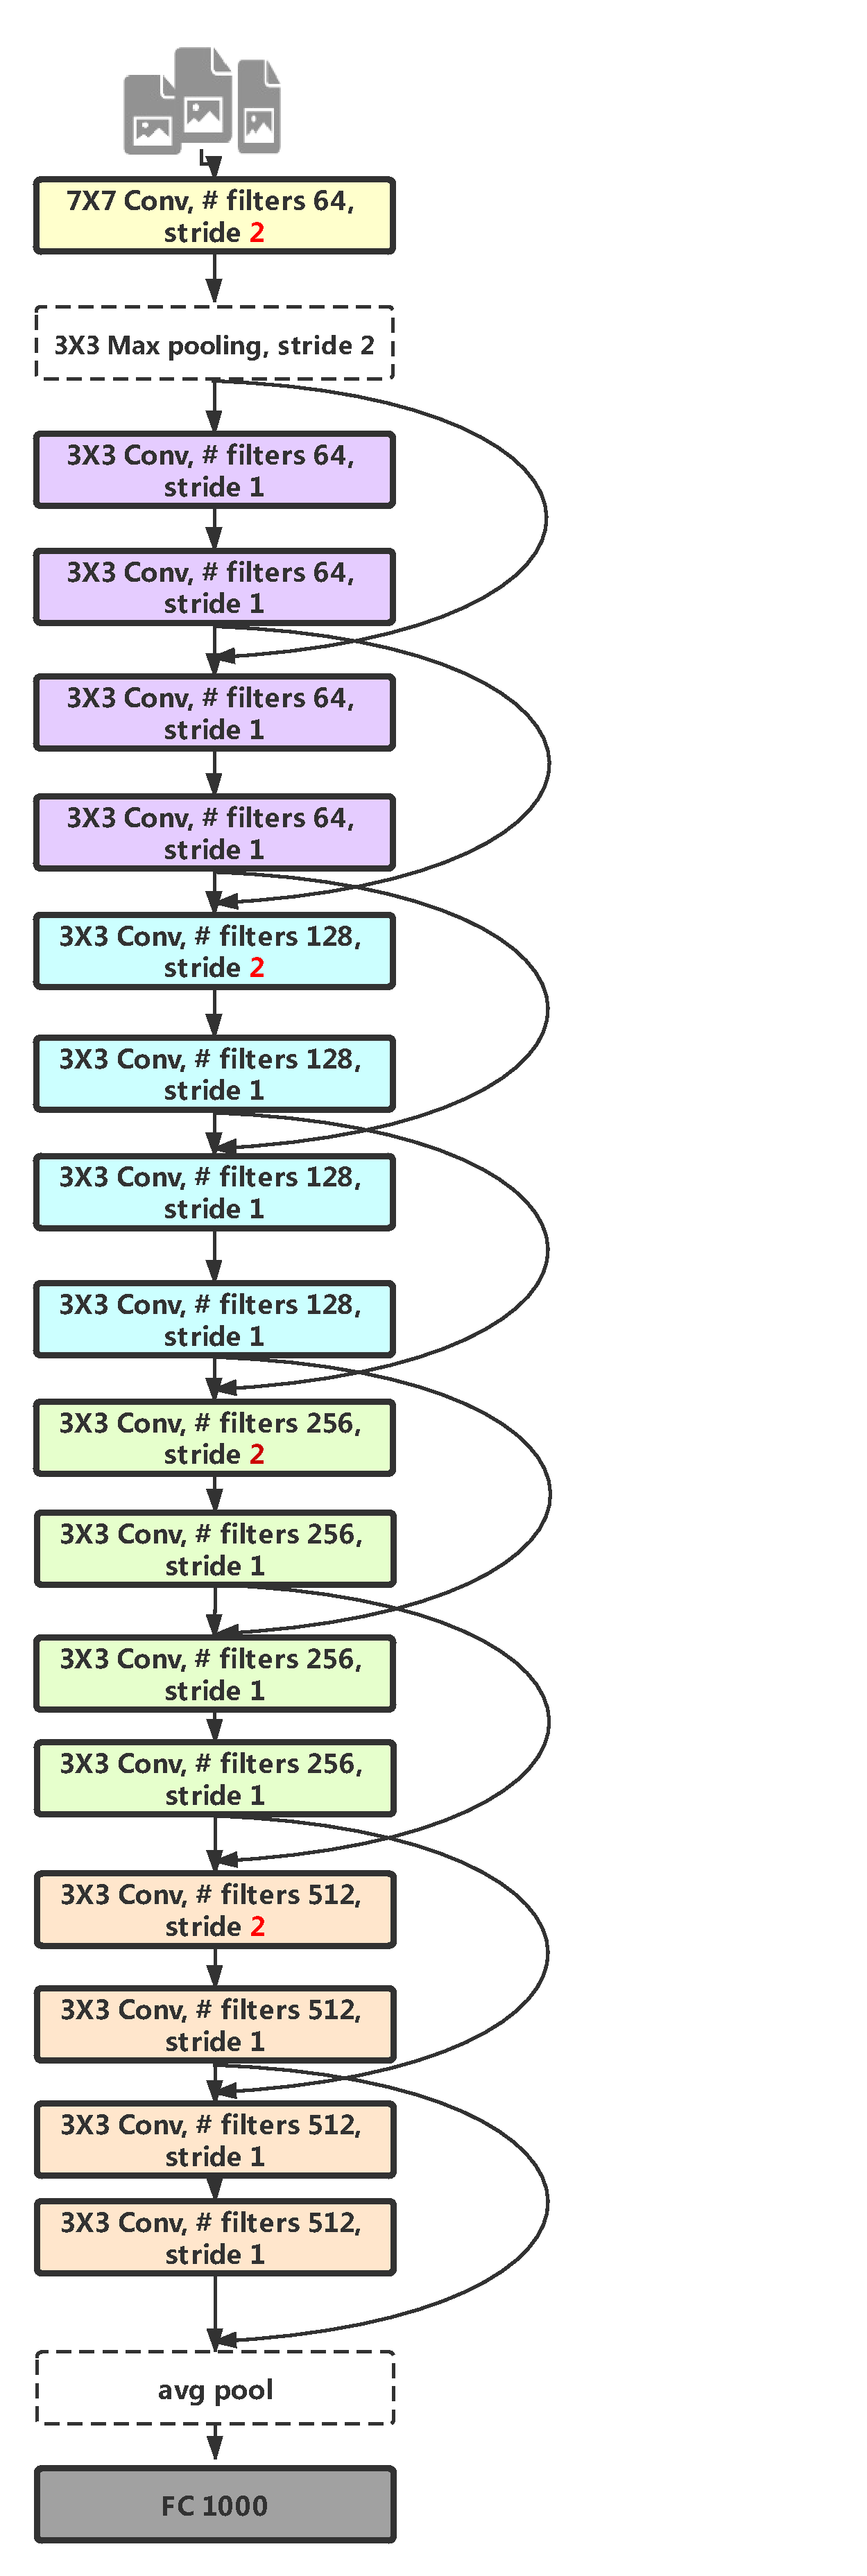
\includegraphics[height=6.5in]{thesis-template-master/images/res18.pdf}
			\caption{Overall architecture of ResNet18}
			\label{fig:res18}
		\end{subfigure}
		\begin{subfigure}[t]{0.49\textwidth}
		    \centering
			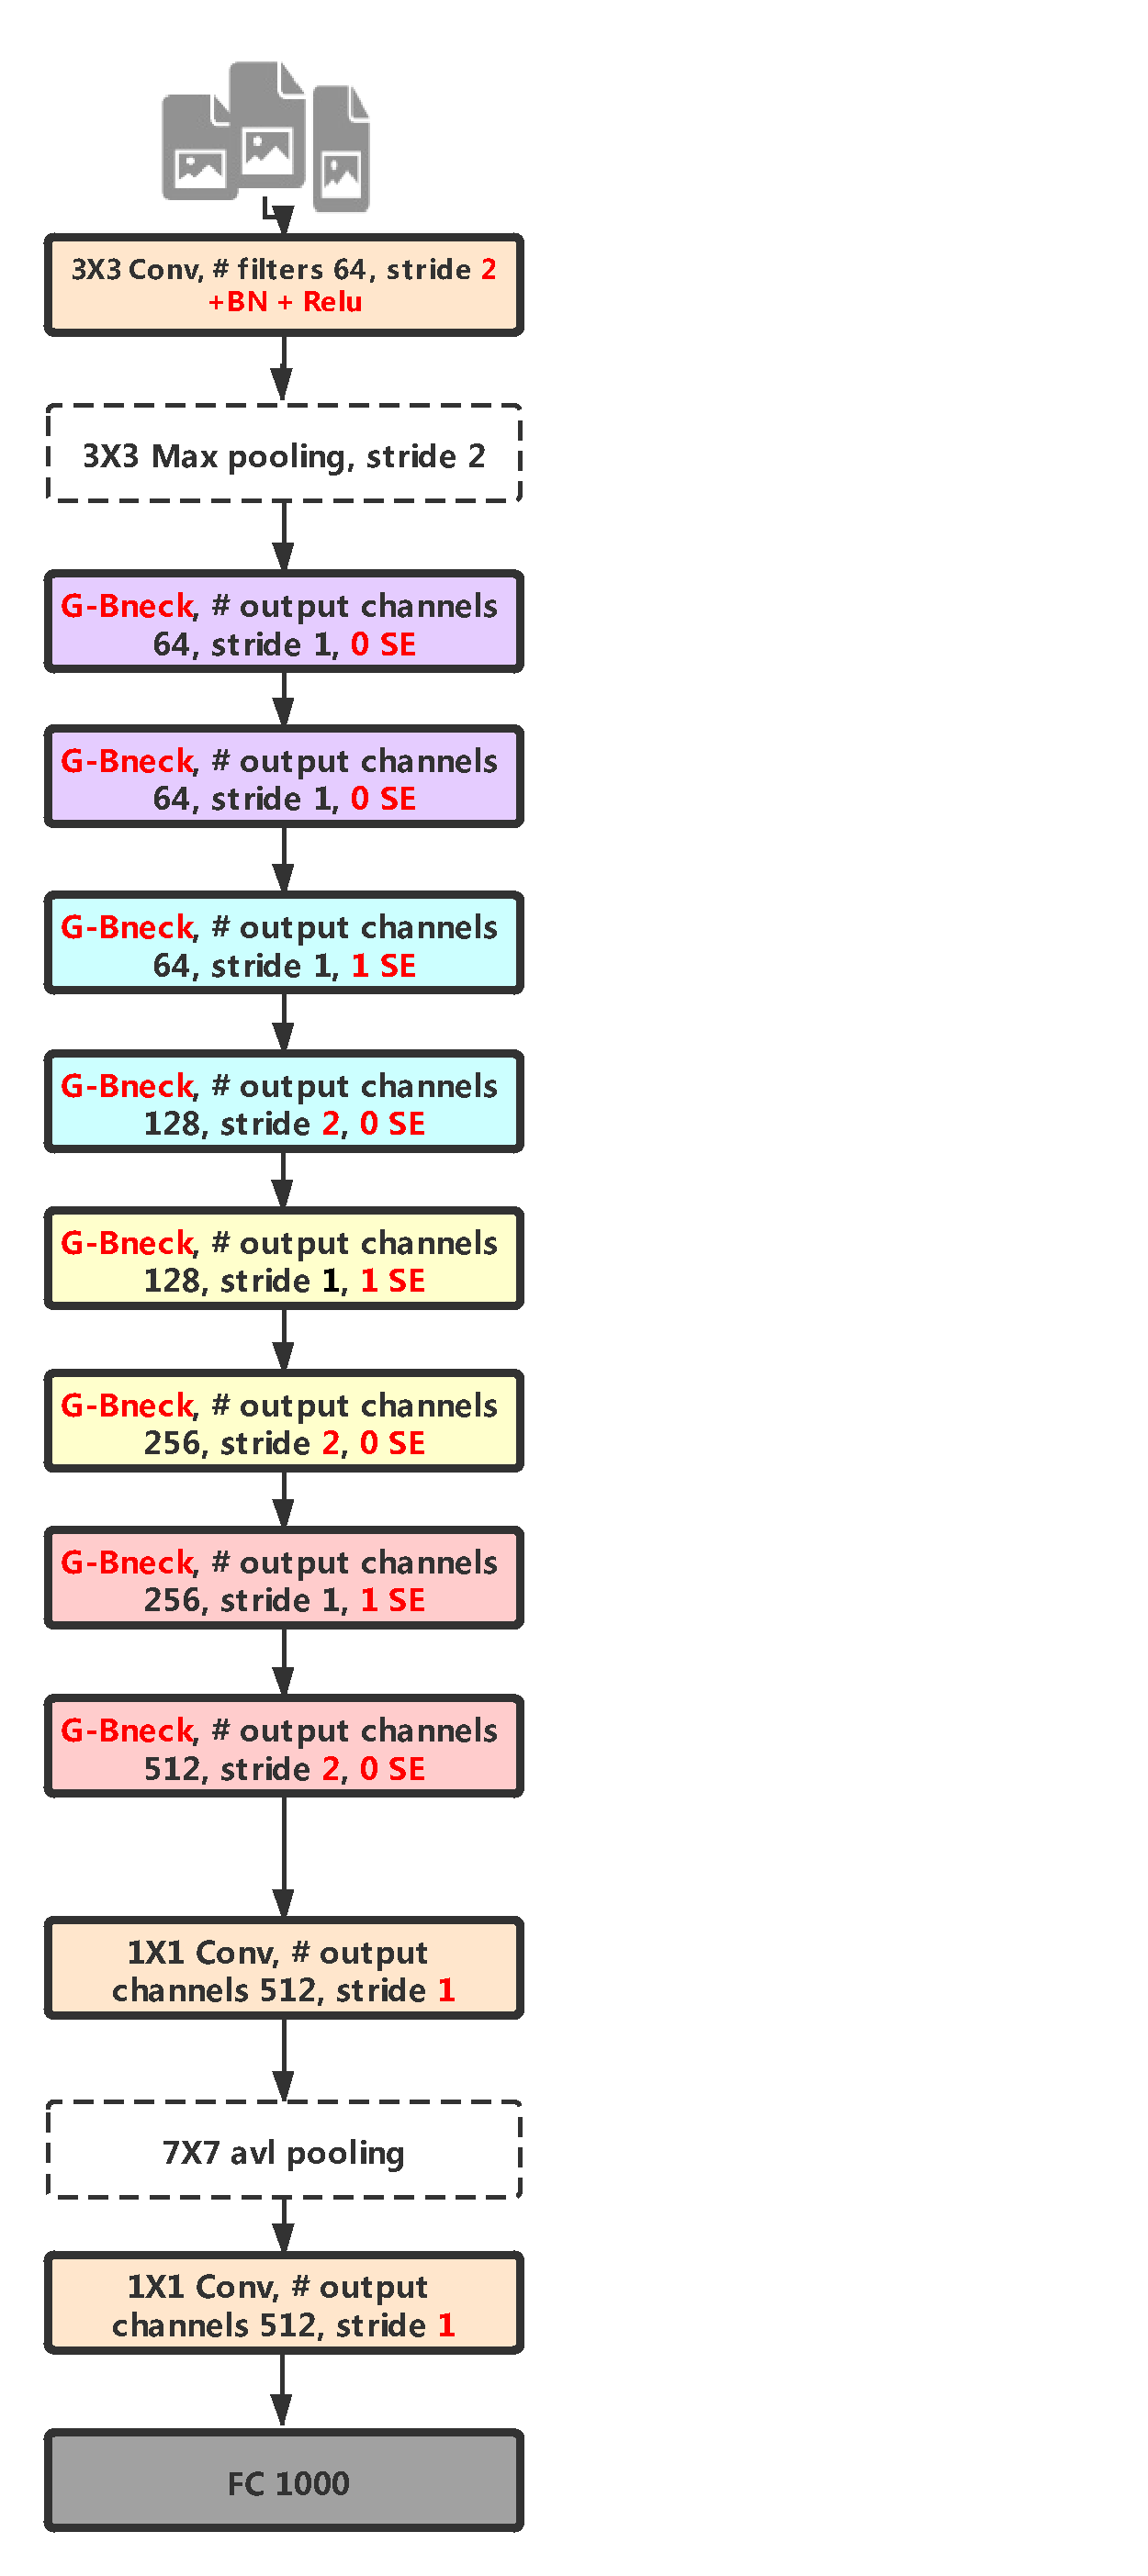
\includegraphics[height =6in]{thesis-template-master/images/Ghostres18.pdf}
			\caption{Overall architecture of CellNet}
			\label{fig:cellnet}
		\end{subfigure}
	\end{center}
	\caption{\textbf{The comparison between ResNet18 \cite{b20} and CellNet}. Despite its simplicity (only 8 layers ghost module) and lower parameters ( $1/4$ weights than ResNet18 \cite{b20}), inside Ghost bottleneck adopted residual function for deeper gradient forward.}
\end{figure}



Inspired by those two outstanding neural network\cite{b19}\cite{b20}, instead of stacking lots of point-wise convolutional layers and taking huge amount of convolutional manipulations, we can avoid the redundant feature maps by cheap operation. 

As shown in Table 1. The first layer of CellNet is a standard convolutional layer with 64 filters, follows standard batch normalization and relu, in order to generate initial intrinsic feature maps, then we purpose a few series of G-bneck, namely 8 layers. In each stage first apply stride = 1 then apply stride = 2 bottleneck which gradually increase the output channel dimension. After 8 layer feature extraction, we get a 512-dimensional feature vector by global average pooling and convolutional layer. SE layer applied to scale less important feature map. Smoothing, blurring and motion are also widely used linear operation, but they need more GPU support. By using depth-wise convolution layer, we can generate more correlated ghost feature maps with cheaper cost.
\begin{table}[htbp]
\centering

\scalebox{0.85}{
\begin{tabular}{@{}llllllll@{}}
\toprule
layer & Type    & Filters & Size/Stride           & Input      & Output     & \multicolumn{1}{l}{\#Expan} & SE \\ \midrule
0     & Conv2d  & 64      & $3\times3$/2                 & 416\times416\times3  & 112\times112\times64 & -                                  & -  \\
1     & Maxpool & -       & $3\times3$/2                 & 112\times112\times64 & 56\times56\times64   & -                                  & -  \\
2     & G-bneck & 64      & $3\times3$/1                 & 56\times56\times64   & 56\times56\times64   & 64                                 & 0  \\
3     & G-bneck & 64      & $3\times3$/1                 & 56\times56\times64   & 56\times56\times64   & 64                                 & 0  \\
4     & G-bneck & 64      & $3\times3$/1                 & 56\times56\times64   & 56\times56\times64   & 128                                & 1  \\
5     & G-bneck & 128     & $3\times3$/2                 & 56\times56\times64   & 28\times28\times128  & 256                                & 0  \\
6     & G-bneck & 128     & $3\times3$/1                 & 28\times28\times128  & 28\times28\times128  & 512                                & 1  \\
7     & G-bneck & 256     & $3\times3$/2                 & 28\times28\times128  & 14\times14\times256  & 1024                               & 0  \\
8     & G-bneck & 256     & $3\times3$/1                 & 14\times14\times256  & 14\times14\times256  & 1024                               & 1  \\
9     & G-bneck & 512     & $3\times3$/2                 & 14\times14\times256  & 7\times7\times512    & 1024                               & 0  \\
10    & Conv2d  & 512     & $1\times1$/1                 & 7\times7\times512    & 7\times7\times512    & -                                  & -  \\
11    & Advpool & -       & 7\times7                   & 7\times7\times512    & $1\times1\times512$    & -                                  & -  \\
12    & Conv2d  & 512     & $1\times1$/1                 & $1\times1\times512$   & $1\times1\times512$    & -                                  & -  \\
13    & FC      & -       & \multicolumn{1}{c}{-} & $1\times1\times512$    & 1000       & -                                  & -  \\ \bottomrule


\end{tabular}}
\caption{\textbf{CellNet Network Structure}. G-bneck denotes novel Ghostbottleneck. \#Expan means expansion size.}
\end{table}

\begin{figure}[h]
	\begin{center}
		\begin{subfigure}[b]{0.49\textwidth}
			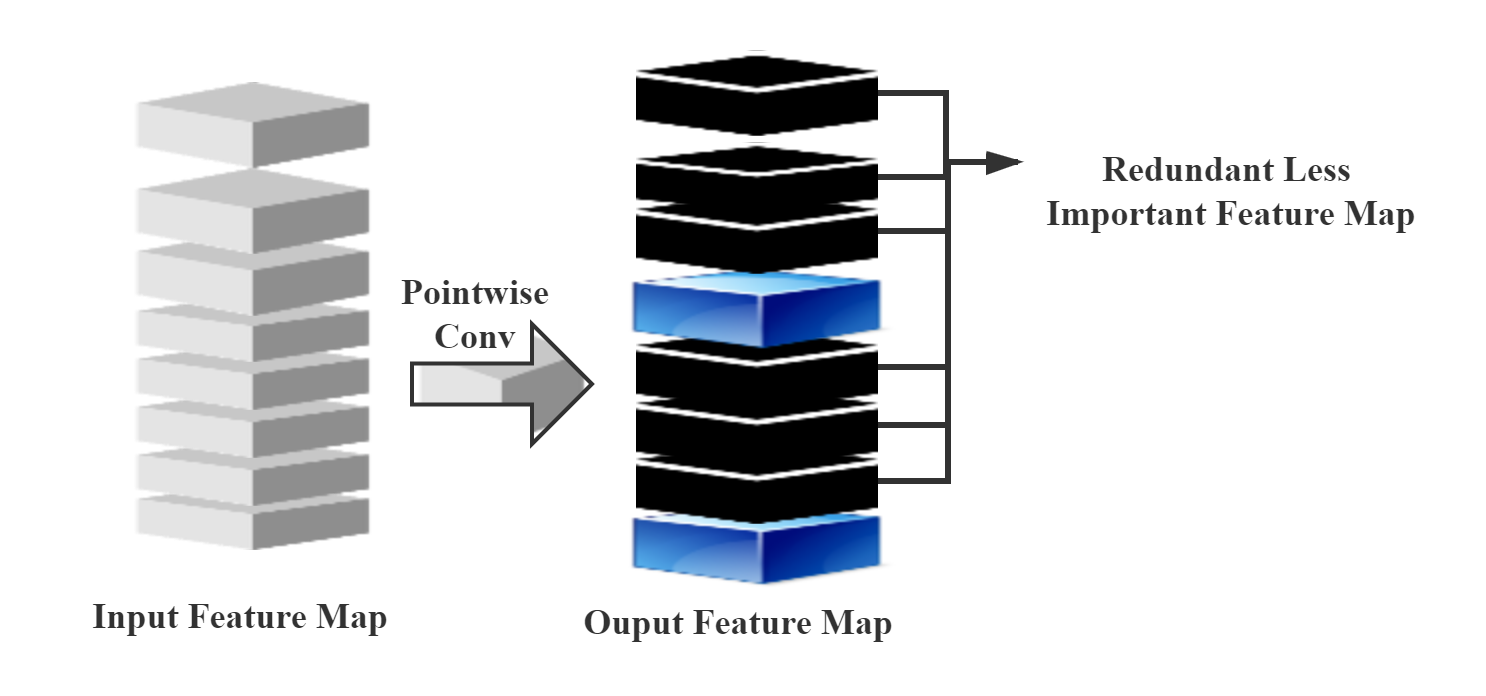
\includegraphics[width=\textwidth]{thesis-template-master/images/normal conv.png}
			\caption{The normal Convolutional layer}
			\label{fig:res18}
		\end{subfigure}
		\begin{subfigure}[b]{0.49\textwidth}
		    \centering
			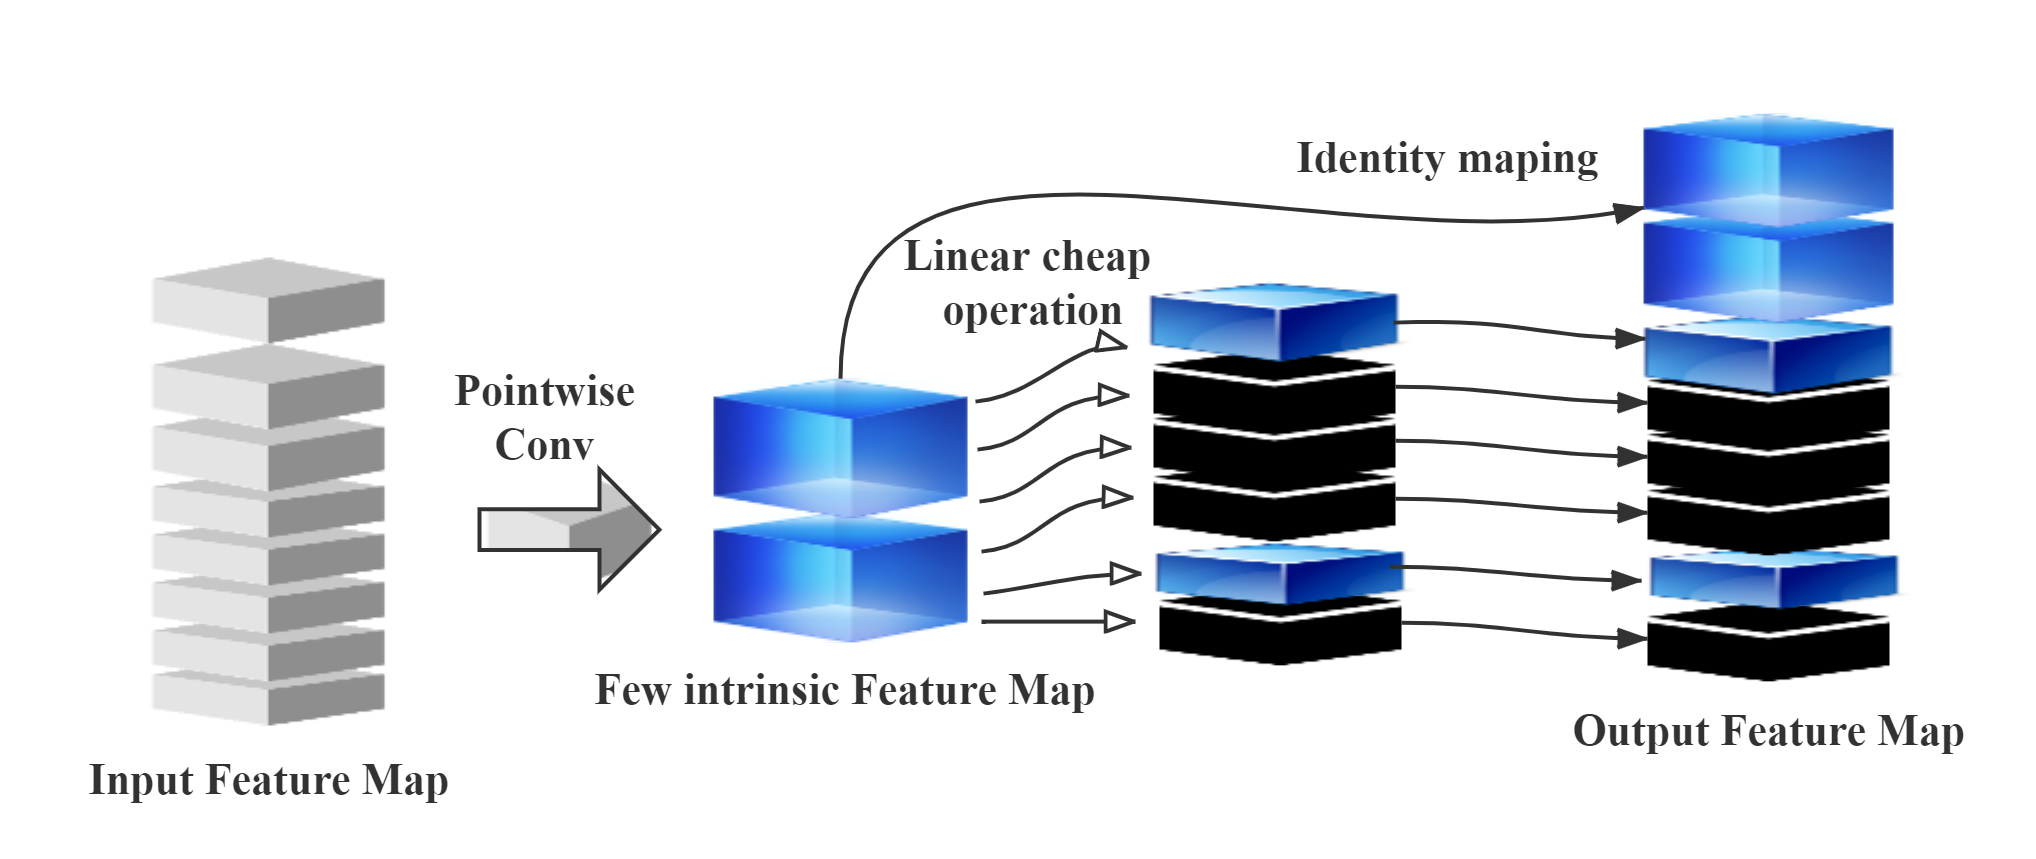
\includegraphics[width=\textwidth]{thesis-template-master/images/ghostmodule.png}
			\caption{The Ghost module}
			\label{fig:cellnet}
		\end{subfigure}
	\end{center}
	\caption{\textbf{The comparison between normal convolutional layer in \cite{b26}\cite{b27}\cite{b28} and ghost module}. We only take point-wise convolution once to get a few intrinsic feature maps, then we utilized the linear cheap transformation to generate ghost map with lower cost.}
\end{figure}



\textbf{Ghostmodule: Is point-wise convolution really indispensable?} Unlike Ghost module applied in GhostNet\cite{b19}, we designed two kind of novel Ghost Modules for feature extraction and adopted the SE layers from Squeeze-and-Excitation Networks \cite{b24} for enhancing useful features and balancing less inhibiting feature map. The first novel Ghost module inside of Gbneck acts as an expansion layer increasing the number of channels, while second Ghost module reduces the number of channels to match the shortcut path. Then the inputs and the outputs of these two Ghost modules are concatenated by shortcut. We adopted batch normalization (BN) and ReLU non-linearity right after each layer as well\cite{b19}, except that ReLU was not used after the second Ghost module as suggested by MobileNetV2\cite{b30}. In each novel Ghost Module, we only take point-wise convolution once to get a few intrinsic feature maps, then we utilized the linear cheap transformation such as depth-wise convolution or affine transformation and wavelet transformation, as suggested by GhostNet\cite{b19}, here the depth-wise convolution was used.

\begin{figure}[h]
	\begin{center}
		\begin{subfigure}[b]{0.49\textwidth}
			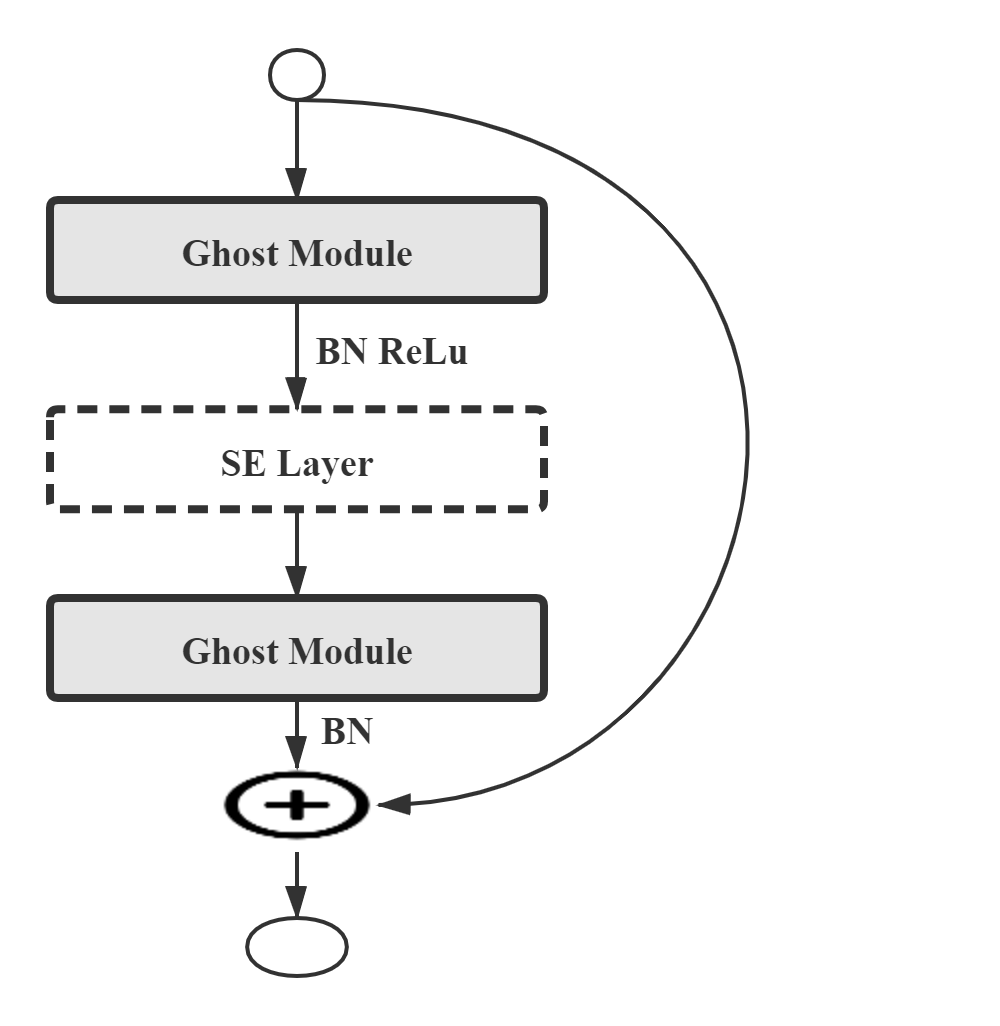
\includegraphics[width=3.5in]{thesis-template-master/images/stride1 module.png}
			\caption{Stride = 1 SE = 0 G-bneck}
			\label{fig:res18}
		\end{subfigure}
		\begin{subfigure}[b]{0.49\textwidth}
			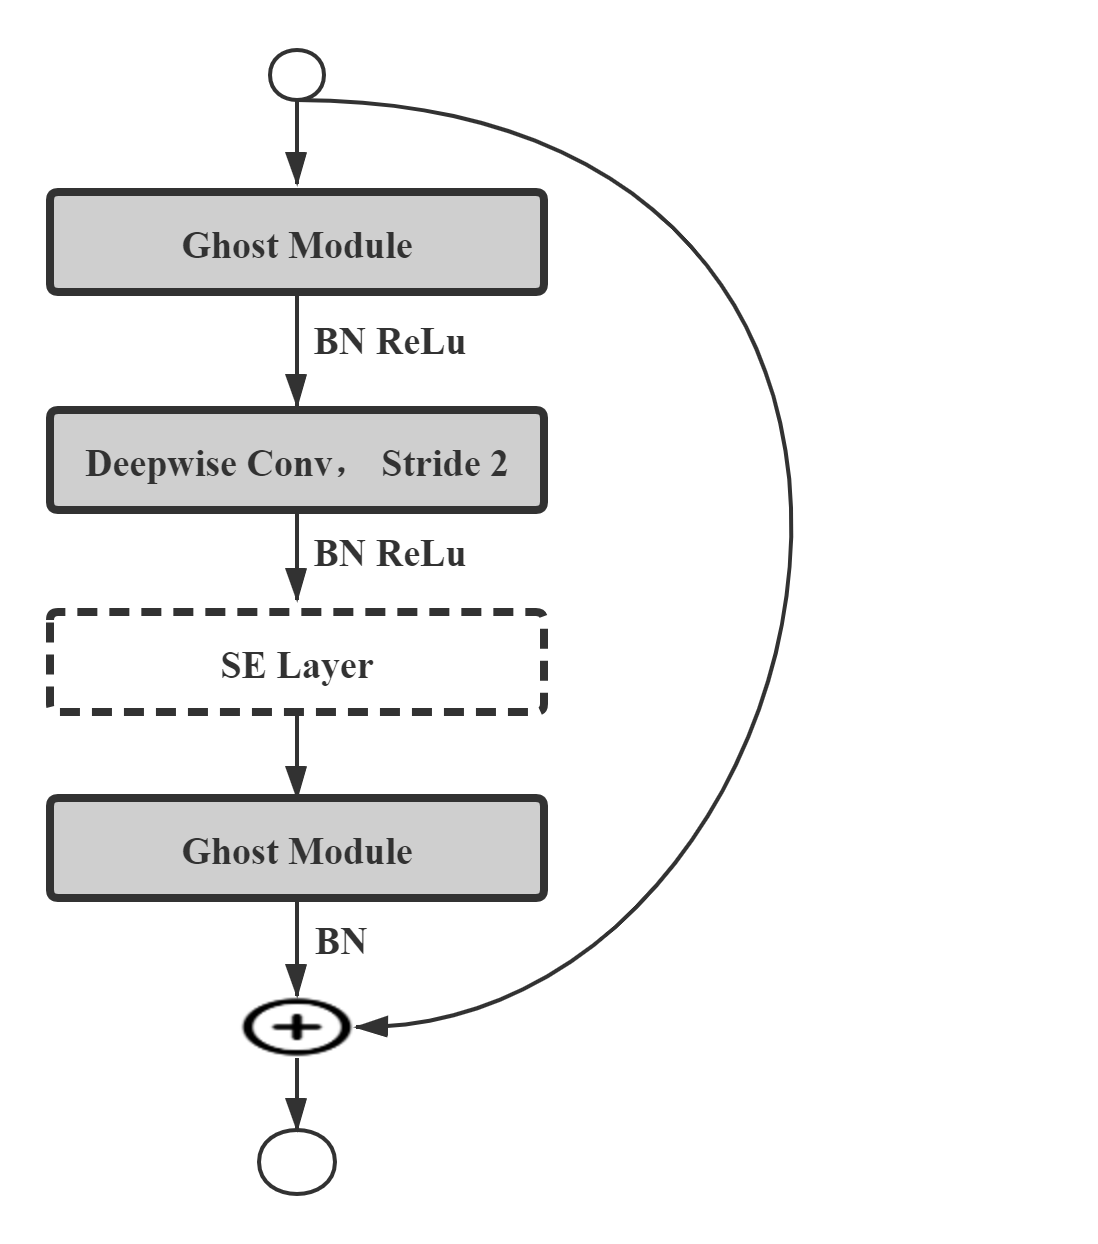
\includegraphics[width=3.5in]{thesis-template-master/images/stride2 module.png}
			\caption{Stride = 2 SE = 0 G-bneck}
			\label{fig:cellnet}
		\end{subfigure}
	\end{center}
	\caption{Two kind of Gbnecks we proposed for feature extraction. where we apply Stride = 1 to keep the output channel of the feature map, Stride = 2 decreases the output channel while extracting information without losing a lot of information. SE = 0 represents not applying SE layer.}
\end{figure}


\textbf{Squeeze-and-Excitation(SE Layer): scaling inhibiting vs intrinsic features map.} Squeeze-and-Excitation (SE)\cite{b24} adaptively recalibrates channel-wise feature responses by explicitly modeling inter-dependencies between channels. 



\subsubsection{Analysis on complexities and necessities}
Here, we further analyze the profit on memory usage and theoretical speed-up by employing the Ghost module, in additional we will plot the visual experiments. The theoretical speed-up ratio $\gamma$ of upgrading ordinary convolution with the Ghost module is equal to following:

\begin{equation}
\begin{split}
\gamma $& = \frac{\left ( n\cdot {h}'\cdot {w}'\cdot c\cdot k\cdot k \right )}{\left (\frac{n}{s}\cdot {h}'\cdot {w}'\cdot c\cdot k\cdot k +\left ( s-1 \right )\cdot \frac{n}{s}\cdot {h}'\cdot {w}' \cdot d\cdot d \right )} \\
$&= \frac{c\cdot k\cdot k}{\frac{1}{s}\cdot c\cdot k\cdot k + \frac{s-1}{s}\cdot d\cdot d } \\
$&\approx \frac{s\cdot c}{s +c-1 } \\
$&\approx s $\label{speed}
\end{split}
\end{equation}

In Equation \eqref{speed}, ${h}' \cdot {w}' \cdot {n}$ represents  $n$ output feature maps with height ${h}'$, width ${w}'$, and $k \cdot k$, $d \cdot d$ stands for the convolution kernel filter and linear operation kernel size, respectively. And $m$ is the number of intrinsic feature maps, where $m < n$ because we only take few intrinsic feature maps and apply a series of cheap linear operations on each intrinsic feature to generate $s$ ghost features. It is also noteworthy that there are 1 ghost map adopted by identify mapping that indicates $s-1$. In total there are $\frac{n}{s} \cdot(s-1)$  linear operations. This leads to theoretically $s$ speed-up ratio.

More feature maps generated by linear operation based on a set of intrinsic feature maps, instead of generating a lot of redundant data by point-wise convolution which takes huge amount of parameters simultaneously. This also partially explains that our net achieves the best performance on several benchmarks shown in Table 2 and Table 3.
As far as we deeply analyze each-layer-generated feature map by our net, we can also figure out the second factor: the artifacts appear in the image could also be learned by the neural network, which greatly affects the accuracy of the network, with the combination of AttentionNet segmentation techniques in cell image pre-processing, we can more focus on object rather than artifacts.


\begin{table}[h]
\centering
\begin{tabular}{@{}llll@{}}
\toprule
Model     & \begin{tabular}[c]{@{}c@{}}Weights\\ (million)\end{tabular} & \begin{tabular}[c]{@{}c@{}}Top-1 Val Acc.\\ (\%)\end{tabular} & \begin{tabular}[c]{@{}c@{}}FLOPs\\ (million)\end{tabular} \\ \midrule
VGG-16\cite{b23}    & 15                                                          & {\color[HTML]{CB0000} \textbf{93.6}}                          & 313                                                       \\
ResNet18\cite{b20}   & 11                                                          & 88.779                                                        & 180                                                       \\
Ghost Net\cite{b19} & 5.18                                                        & 88.238                                                        & 141                                                       \\
*our      & {\color[HTML]{CB0000} \textbf{2.91}}                        & {\color[HTML]{333333} \textbf{92.45}}                         & {\color[HTML]{CB0000} \textbf{41.7}}                      \\ \bottomrule
\end{tabular}
\caption{\textbf{Comparison of structure and parameters of state-of-the-art methods on Cifar10 dataset}}
\end{table}


\begin{table}[h]
\centering
\begin{tabular}{@{}llll@{}}
\toprule
Model                                                  & \begin{tabular}[c]{@{}l@{}}Weights\\ (million)\end{tabular} & \begin{tabular}[c]{@{}l@{}}Top-1 Val Acc.\\ (\%)\end{tabular} & \begin{tabular}[c]{@{}l@{}}FLOPs\\ (million)\end{tabular} \\ \midrule
\begin{tabular}[c]{@{}l@{}}Inception V3\cite{b38}\end{tabular} & 23.81                                                       & 88.0                                                          & 540                                                       \\
ResNet18\cite{b20}                                               & 11                                                          & 87.50                                                         & 180                                                       \\
Ghost Net\cite{b19}                                              & 5.18                                                        & 88.69                                                         & 141                                                       \\
*our                                                   & {\color[HTML]{CB0000} \textbf{2.91}}                        & {\color[HTML]{CB0000} \textbf{91.78}}                         & {\color[HTML]{CB0000} \textbf{41.7}}                      \\ \bottomrule
\end{tabular}
\centering
\caption{\textbf{Comparison of structure and parameters of state-of-the-art methods on Pneumonia dataset}}
\end{table}

\begin{figure}[h]
	\begin{center}
		\begin{subfigure}[b]{0.45\textwidth}
		    \centering
			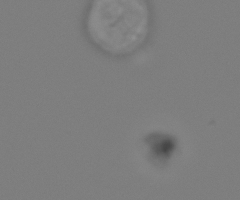
\includegraphics[height= 0.10\textheight]{thesis-template-master/images/hd1 (4400).png}
			\caption{}
			\label{fig:res18}
		\end{subfigure}
		\begin{subfigure}[b]{0.45\textwidth}
		    \centering
			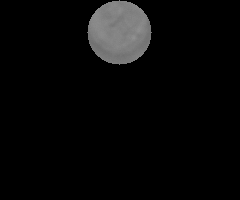
\includegraphics[height= 0.10\textheight]{thesis-template-master/images/hd1 (4400) (1).png}
			\caption{}
			\label{fig:cellnet}
		\end{subfigure}
		
		\begin{subfigure}[b]{0.45\textwidth}
		    \centering
			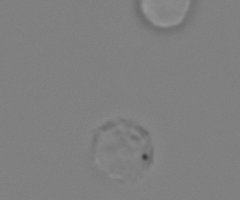
\includegraphics[height= 0.10\textheight]{thesis-template-master/images/hd1 (4550).png}
			\caption{}
			\label{fig:cellnet}
		\end{subfigure}
		\begin{subfigure}[b]{0.45\textwidth}
		    \centering
			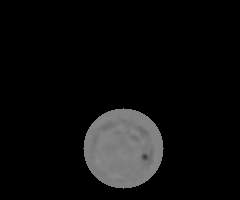
\includegraphics[height= 0.10\textheight]{thesis-template-master/images/hd1 (4550) (1).png}
			\caption{}
			\label{fig:cellnet}
		\end{subfigure}
		\begin{subfigure}[b]{0.45\textwidth}
		    \centering
			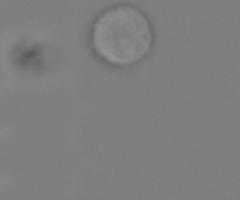
\includegraphics[height= 0.10\textheight]{thesis-template-master/images/ss2_8 (142).png}
			\caption{}
			\label{fig:cellnet}
		\end{subfigure}
		\begin{subfigure}[b]{0.45\textwidth}
		    \centering
			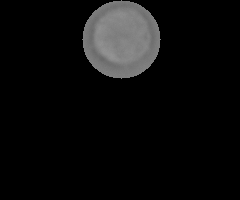
\includegraphics[height= 0.10\textheight]{thesis-template-master/images/ss2_8 (142) (1).png}
			\caption{}
			\label{fig:cellnet}
		\end{subfigure}
		
		
		\begin{subfigure}[b]{0.33\textwidth}
		    \centering
			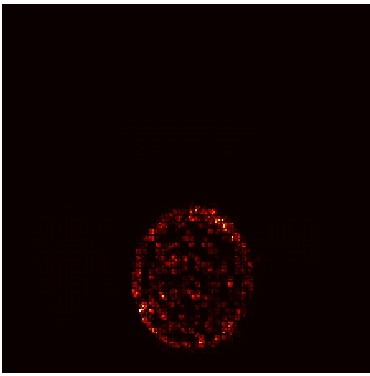
\includegraphics[height= 0.20\textheight]{thesis-template-master/images/hd1 (4550)ournetWithcellyolo.jpg}
			\caption{}
			\label{fig:cellnet}
		\end{subfigure}
		\begin{subfigure}[b]{0.33\textwidth}
		    \centering
			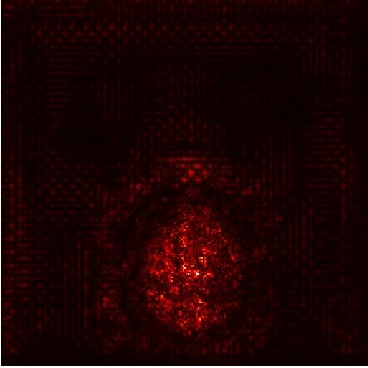
\includegraphics[height= 0.20\textheight]{thesis-template-master/images/hd1 (4550)resnetWithcellyolo.jpg}
			\caption{}
			\label{fig:cellnet}
		\end{subfigure}
		\begin{subfigure}[b]{0.33\textwidth}
		    \centering
			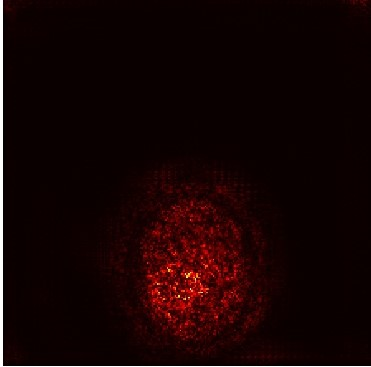
\includegraphics[height= 0.20\textheight]{thesis-template-master/images/hd1 (4550)vggnetWithcellyolo.jpg}
			\caption{}
			\label{fig:cellnet}
		\end{subfigure}
	\end{center}
	\caption{The illustration of the necessity of Ghost-Module and AttentionNet. (a)-(f) implying the performances of AttentionNet. After AttentionNet segmentation, artifacts will be removed and only morphological characteristics of the objects stay. The second row are saliency map of cell (d) after ResNet18\cite{b20} (h), our Net (g) and VGG16 net \cite{b23} (i). Leading  STOA  algorithms, such ResNet18 and VGG16 net, are  more focus  these  non  ROI  features,  such  as  the  debris  feature  outside the ROI. Those leading networks pay more attention to those debris information leads to worse classification performance.}
\end{figure}

\begin{figure}[h]
	\begin{center}
		\begin{subfigure}[b]{0.49\textwidth}
			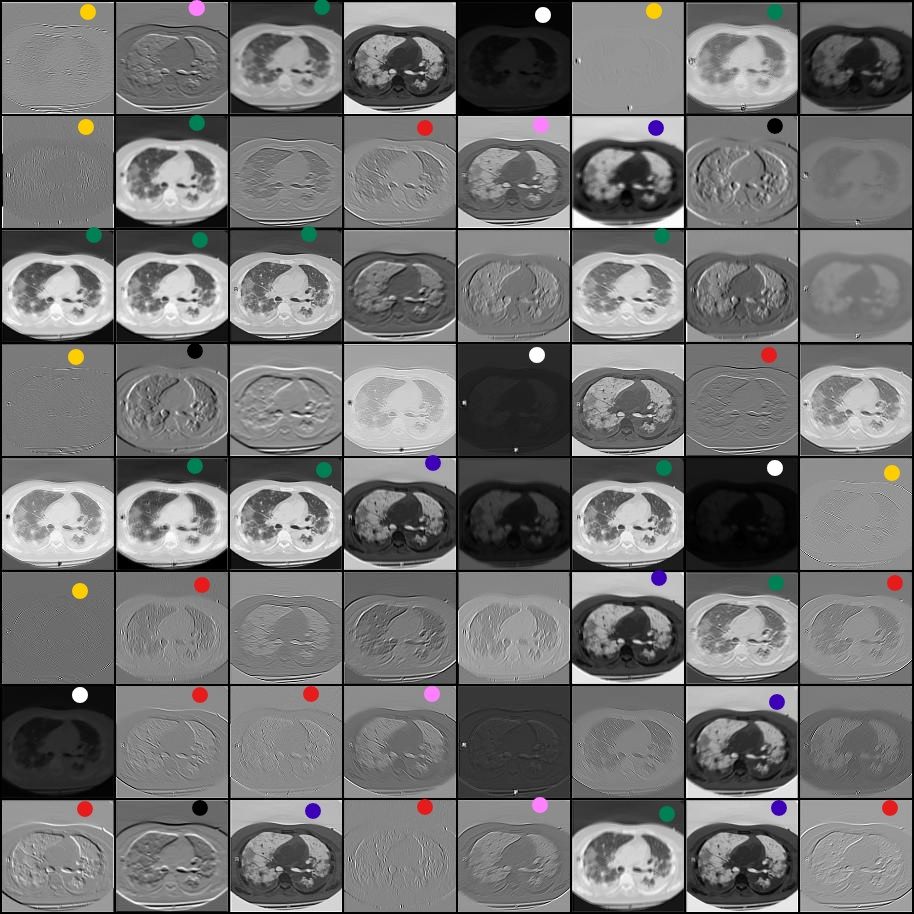
\includegraphics[height= 0.25\textheight]{thesis-template-master/images/Inkedfirst Conv1 of resnet18 with pretrain weights on coviddataset_LI.jpg}
			\caption{}
			\label{fig:res18}
		\end{subfigure}
		
		
		\begin{subfigure}[b]{0.49\textwidth}
			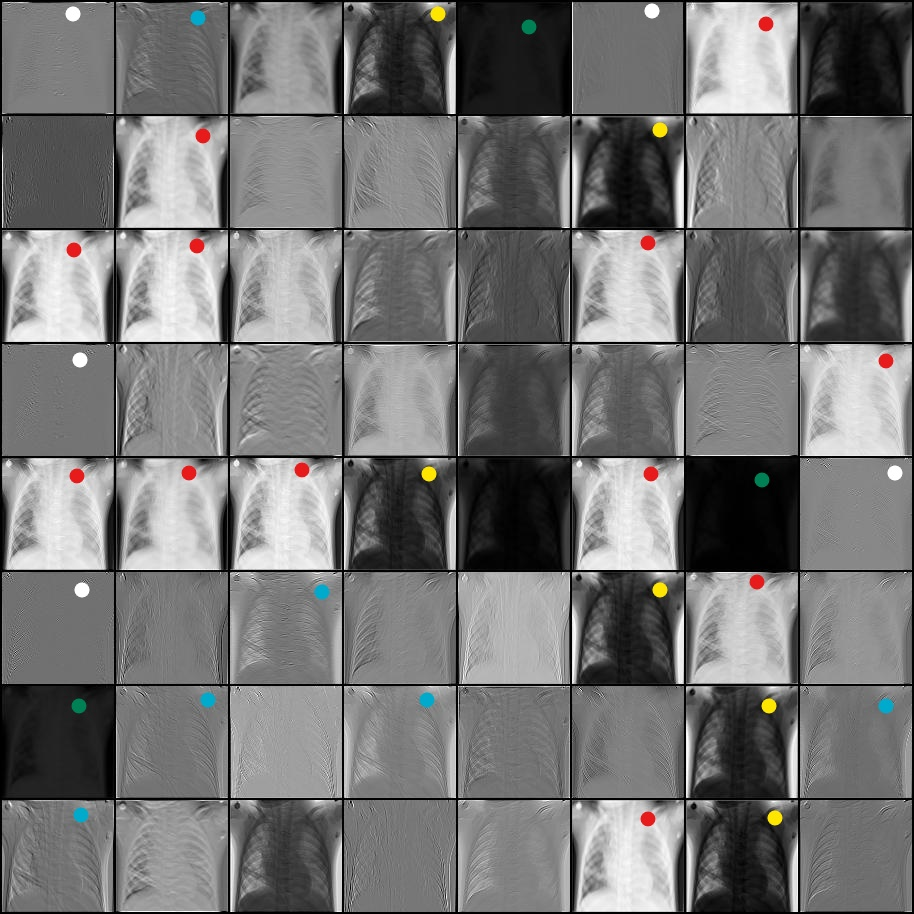
\includegraphics[height= 0.25\textheight]{thesis-template-master/images/Inkedfirst Conv1 of resnet18 with pretrain weights on penudataset_LI.jpg}
			\caption{}
			\label{fig:cellnet}
		\end{subfigure}
		
		\begin{subfigure}[b]{0.49\textwidth}
			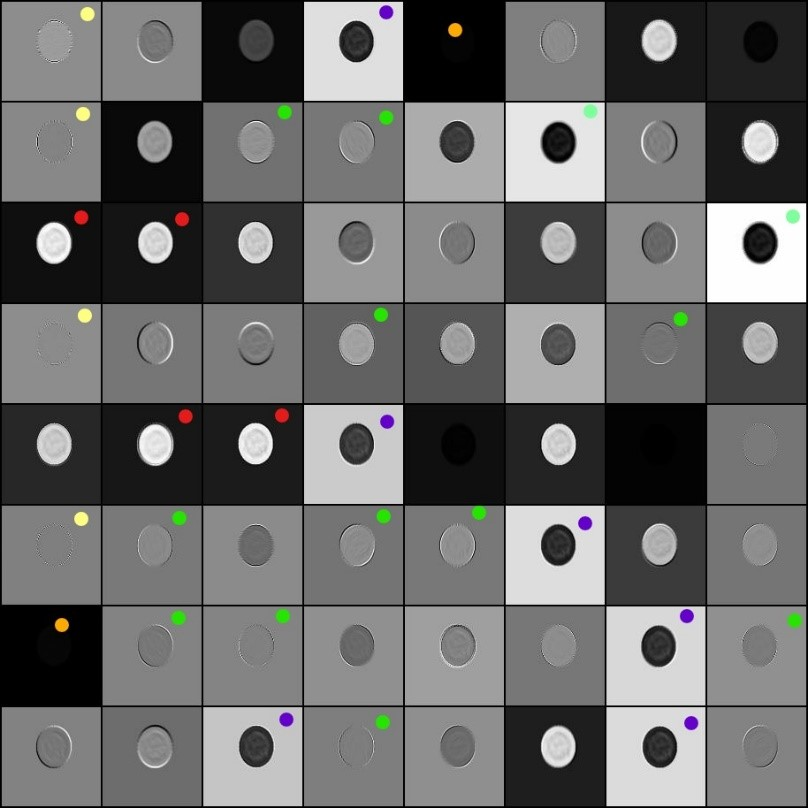
\includegraphics[height= 0.25\textheight]{thesis-template-master/images/cellnetnecc3.jpg}
			\caption{}
			\label{fig:cellnet}
		\end{subfigure}
		
	\end{center}
	\caption{The illustration of the necessity of Ghost-Module and CellNet. There are visualization of feature maps after ResNet18\cite{b20} 1st convolutional layer. Whether it is a Xray image of COVID-19 dataset (a), a cell image segmented by attentation (c), or a CT image from Pneumonia Dataset (b), after the first layer of point-wise convolution there is a large amount of redundant feature maps (see the same color marked). Especially for Sezary Syndrome Dataset, there is no need to operate point-wise convolution one by one after AttentionNet segmentation, because all the valid information is within the circle.}
\end{figure}

\subsubsection{AttentionNet: Automatic Detector and Segment-or}\label{AA}
The proposed AttentionNet follows basic structure of YOLOv3-tiny algorithm\cite{b33}, and it attempts to process more efficiently on small target. The attributes of self-detection and labeling, of nearly real-time resolve and of general resource requirements mainly characterize the AttentionNet Network. At the beginning it is  similar to YOLOv3\cite{b33} that the input image is divided into an $M \times M$ grid. Then $B$ bounding boxes and confidence score are defined in each grid cell. Each grid cell predicts $C$ conditional probabilities, denoted as $P(Class_{i}\mid Object_{j})$ for $i$ classes and object $j$. If there is an object $j$ in the grid, then indicated the objectiveness score $P(Object_{j})$  equal to $1$\cite{b18}. Here, we refer the initiatives from YoloV3, the confidence score also represents the accuracy of the box prediction, which is defined as $GIOU_{Ground truth}^{Predition}$. Unlike the originally YOLOv3\cite{b33}, instead of using Intersection‐Over‐Union (IOU), we use $GIOU$ with higher precision, which refers to the generalized intersection area between the predicted bounding box and ground truth box.

It should be noted that each grid cell predicted conditional class probability is not same as the confidence score. These often leads to misunderstanding of the fact that the former $P(Class_{i} \mid Object_{j})$ is predicted in each grid, while the $P(Object_{j}) \times GIOU_{Ground truth}^{Predition}$ is predicted in each bounding box\cite{b18}. 
Finally Class Score $S$ is defined as follow (1): \label{eq}
\begin{equation}
\begin{split}
$S&=P(Class_{i}\mid Object_{j}) \times P(Object_{j}) \times GIOU_{Ground truth}^{Predition} \\
$& = P(Class_{i}) \times GIOU_{Ground truth}^{Predition} $\label{eq}
\end{split}
\end{equation}

The Class Score $S$ computed the probability of the object $j \in  i$ class appearing in the box, as well as how well the bounding box fits each object $j$.

The original YOLOv3\cite{b33} used the darknet front-end feature extraction module, but the detection performance on Sezary Syndrom dataset is unsatisfied. On the contrary, AttentionNet with only $13 \times 13$, $26 \times 26$ yolo scale output tensors adopts multi-scale fusion, and K means++ clustering\cite{b18} techniques, outperforms TF-Yolo\cite{b18} and  YOLOv3 \cite{b33}, which has $13 \times 13$, $26 \times 26$, $52 \times 52$ yolo scale output tensor. In order to train a suitable segment-or, it is recommended to choose corresponding scale tensors refer to different data sets. 

\textbf{GBCIOU and Circle segmentation.} Using the cvfillPoly function, we can easily classify the cell image into simple polygonal areas and achieve high-speed segmentation once we obtain the output from AttentionNet network for anchor box detection, namely ( $x_{1}$, $y_{1}$, $x_{2}$, $y_{2}$). However, it has very obvious shortcomings that the shape of the segmentation does not perfectly approximate the ground truth of the cell. To overcome this problem, we proposed $HSV$ space mask threshold method, simply converting to $HSV$ space and using threshold to eliminate the outside part of central circle of box detection.  For the common challenge of the YOLO original version: when multiple objects standing in the same area or overlapping in the central point, it will become much more difficult to draw the correct prediction and always leads to wrong labeling. In our case if multiple cells occur and one cell has more competitive confidence score than another during circle detection that will leads to either non-labelled or partly labelled problem.
We proposed the GBCIOU function to ideally find general intersected box center when multiple box predictions occur in the same image, in addition to the GIOU (general interaction of union) computes the deviation between ground truth and the prediction.



\subsection{Experiments}
To verify the effectiveness of the proposed novel Ghost module and CellNet architecture, we conduct experiments on several benchmark visual datasets, including CIFAR-10\cite{b21}, phenomenon dataset \cite{b38}, and COVID-19 benchmark \cite{b36}\cite{b37}. 


\subsubsection{CellNet on Visual Benchmarks}



\begin{figure}[h]
\centering
\includegraphics[height=200pt, width=0.9\textwidth]{thesis-template-master/images/Cifar-12-06-2020.png}
\label{fig}
\centering
\caption{Comparison of state-of-art methods for training on benchmark CIFAR-10 Dataset. Our Net can achieve higher classification performance  (e.g.  92.45\%  Top-1  accuracy ) than both ResNet and GhostNet, it is illustrated by both the standard derivation, namely the stability, and the final converged accuracy.}
\end{figure}
CIFAR-10 dataset\cite{b21} consists of 60,000 $32 \times 32$ color images in 10 classes, with 50,000 training images and 10,000 test images. A common data augmentation scheme including random crop\cite{b22} and mirroring\cite{b19} is adopted as well. Our Net can achieve higher classification performance  (e.g.  92.45\%  Top-1  accuracy  ) than both ResNet18 and GhostNet, with the least  weights, namely $1/7$ weights than VGG16 \cite{b23}. 




On benchmark Pneumonia Dataset\cite{b38}. The Pneumonia / Normal classification val accuracy of our Net converges into nearly 91.785\% better than GhostNet and ResNet18. In addition, after around 80 epochs the accuracy of our Net converges into nearly 91.785\%, comparing to  Inception V3 after 7,000 epochs reaches 88.0\%\cite{b38}.
\begin{figure}[h]
\centering
\includegraphics[height=200pt, width=0.9\textwidth]{thesis-template-master/images/Pneumonia_TimeSeries-1.png}
\label{fig}
\centering
\caption{ Comparison of state-of-art methods for training on Pneumonia Dataset. Benchmark Pneumonia Dataset contains 5,856 Xray/CT images. Considering the fact that Our Net has only 8 Novel Ghostmodule layers and 2.91 millions of weights, outperforms both ResNet18, GhostNet and InceptionV3 net from Accuracy and Complexity perspective views.}
\end{figure}

\begin{figure}[h]
\centering
\includegraphics[height=200pt, width=0.9\textwidth]{thesis-template-master/images/COVID-19_TimeSeries-1.png}
\label{fig}
\centering
\caption{ Comparison of state-of-art methods for training on COVID-19 Dataset.  The weights of our models is 2.91 million, comparing to DenseNet121 7.98 millions of weights, MobileNet V2 3.4 millions of weights and 301 millions of FLOPs. Considering the fact of the higher complexity and parameter amount of other SOTA Nets, our Net is very competitive on classification tasks for the biomedical dataset. }
\end{figure}


\begin{figure}[h]
\includegraphics[height=240pt,width=0.9\textwidth]{thesis-template-master/images/BarDiagram_Bold.png}
\label{fig}
\centering
\caption{Graphical summary of composition of COVID-19 Xray/CT images. Based on initial COVID-19 Image Data Collection \cite{b37}, we additionally collected and sorted nearly 2,000 CT/Xray images, with wide range in gender, age, survival condition and country/places from newest publications and CDC public sources\cite{b36}\cite{b37}\cite{b38}. }
%\caption{Graphical summary of Alex Net\cite{b31}, Squeeze net\cite{b24}, ResNet18\cite{b20}, MobieNetv2\cite{b30}, Our Net, Ghost Net\cite{b19}, DenseNet121\cite{b32}, and Vgg11\cite{b23} performance on COVID-19 dataset. }
\end{figure}
The 2019 novel corona virus (COVID-19) brings huge challenge to our life and we are facing an increasingly disrupted challenging time. In order to help the medical scientists, we made this COVID-19 dataset. Based on initial COVID-19 Image Data Collection\cite{b37}, which contains only 123 frontal view X-rays. We additionally collected data from newest publications and  assembled medical images from websites and publications such as European Journal of Radiology\cite{b36}, and collected nearly 1583 healthy Lung CT images as comparative data from recently available resources and publications\cite{b37} \cite{b38}. COVID-19 Dataset contains nearly 2,000 Xray/CT images we sampled from newest publications. Our Net achieves 3rd place classification performance among these state-of-art models while least weights and computational cost.




\subsection*{Conclusion}
To reduce the complexity and computational costs of recent deep neural networks on biomedical image processing area \cite{b3}\cite{b15}\cite{b17}, this paper presents a novel unifying approach: firstly adopted AttentionNet as a very effective and efficient tool for image pre-processing and artifacts elimination. The experiments conducted on benchmarks illustrate that the AttentionNet method is a plug-and-play tool for SOTA module data pre-processing with remarkable speed and comparable performance. More importantly, we proposed CellNet for biomedical image classification, which using two novel designed Ghost modules to generated ghost feature map that get rid of complex and redundant feature map with lower cost, and it outperforms state-of-the-art neural architectures in several classical medical benchmarks.
What's more, we completed an AI-assisted diagnostic in a real-world medical scenario by integrating 12 leading models (including our AttentionNet and CellNet) into a software application, which provides a reference for high-precision bio-medically assisted diagnosis of complex medical data sets (such as Sezary Syndrome) and all code are publicly available.




\section{CellNet Software}
\label{sec:ipsum}
Mauris ultrices commodo risus, mollis congue dui scelerisque elementum. Nam ac dictum augue. Vestibulum convallis vel dui et porttitor. Aenean a commodo justo. Integer condimentum pulvinar massa, eu venenatis metus bibendum aliquam. Aenean ac tristique nisl, ut maximus tortor. Duis venenatis ultricies tellus, non dignissim metus feugiat vel. Curabitur a lorem ligula. Nunc commodo erat id mauris condimentum euismod. Etiam vel sodales augue. Donec id tincidunt tellus. Pellentesque tempus ultricies lobortis. Vestibulum magna velit, iaculis rhoncus aliquet sed, congue vitae risus. Suspendisse iaculis, nibh at imperdiet tincidunt, mi metus pharetra tortor, quis posuere est ante id ex.

\subsection{Dolor sit} % (fold)
\label{sub:dolor_sit}
Fusce a tortor sit amet quam suscipit commodo non eget massa. Vestibulum semper accumsan tristique. Aenean posuere laoreet sollicitudin. Vivamus nec ligula et nunc ornare pellentesque. Aenean vulputate vestibulum risus facilisis condimentum. Morbi ac ex magna. In feugiat ligula in nisi tincidunt malesuada. Morbi convallis nunc id nisi ultrices venenatis. Donec in felis vel lectus lobortis malesuada. Morbi ut neque nulla. Quisque augue nibh, tempor in elit at, convallis gravida enim. Integer iaculis nibh eget commodo mollis. Vivamus at viverra eros. Pellentesque eu elit velit. Nunc nec ligula diam.

Suspendisse tempus id neque vel ultricies. Vivamus efficitur dui non enim vehicula, sed faucibus massa consectetur. Aenean lacinia sapien quis pellentesque auctor. Vestibulum auctor dui a orci imperdiet, vitae posuere sapien vulputate. In eget augue quis erat rhoncus dignissim ut nec felis. Ut dignissim, ligula a porta sollicitudin, erat enim maximus sapien, vitae vehicula ligula eros sed mauris. Maecenas vehicula, mauris nec sagittis pellentesque, mauris turpis volutpat sapien, vitae mattis magna enim sit amet ligula.

Duis sem elit, egestas eleifend auctor quis, elementum nec nisi. Sed sed ipsum ac mi rutrum pretium. Maecenas a pulvinar eros. Integer eget pretium arcu, at egestas ante. Donec neque magna, pellentesque in justo et, convallis congue enim. Etiam et quam sit amet mi ullamcorper pretium vitae id ligula. Maecenas ac ligula justo. Curabitur gravida nunc tincidunt auctor rhoncus. Donec sit amet ante ipsum. In quis ullamcorper ex. Cras ac ullamcorper orci, et aliquet enim. Nam in elit sit amet tortor finibus interdum.

Sed ac facilisis augue. Cras nec nisl consequat, gravida tortor vitae, tincidunt nisi. Duis posuere eu orci at luctus. Morbi nec malesuada arcu. Aliquam erat volutpat. Maecenas pharetra in nisi sed molestie. Cras id urna eu nunc ullamcorper volutpat a sit amet elit. Donec tincidunt laoreet ipsum, a sagittis tellus laoreet sodales. Aliquam in ultricies sapien, semper tempus nisl. Pellentesque lectus nisi, tempus ut fermentum quis, pulvinar ac velit.

Duis laoreet pellentesque libero, egestas mattis ante maximus id. Donec convallis felis vel neque placerat ornare. Curabitur id iaculis lectus. Duis vitae tristique lectus. Sed maximus aliquet nisl, quis bibendum sem. Vestibulum ut ipsum a risus fermentum dapibus tincidunt semper lorem. Proin ante ante, euismod sed turpis eu, dictum bibendum ipsum. Praesent fermentum volutpat metus, quis fringilla arcu fermentum eget. Suspendisse quis condimentum sapien, ut sollicitudin metus. Ut in volutpat enim. Phasellus sapien est, varius in condimentum et, auctor et augue. Donec mattis malesuada leo, vitae pellentesque metus ornare vel. Pellentesque massa nulla, aliquet nec metus et, auctor porta lacus. Fusce ac ex faucibus, placerat nibh ac, fermentum leo. Curabitur interdum fermentum lacus, quis mollis erat suscipit nec. Vestibulum vel pellentesque ipsum, sit amet ultrices quam.

Proin vestibulum nec risus ut porttitor. Pellentesque porta ipsum elit, quis lacinia quam vehicula eu. Nulla consectetur nulla ac euismod tincidunt. Curabitur quis auctor neque, eget viverra nibh. Vivamus porttitor aliquam leo id iaculis. Cras sed dapibus quam. Mauris ullamcorper lacus ut porta sollicitudin. Proin accumsan finibus dolor, eu suscipit massa interdum non. Maecenas lobortis sit amet leo in fringilla.
% subsection dolor_sit (end)

\subsection{Amet} % (fold)
\label{sub:amet}
Nulla nec accumsan risus. Mauris consectetur ex vel tempus posuere. Quisque sit amet placerat risus, vitae suscipit massa. Maecenas molestie scelerisque ipsum, ac porta purus dapibus ut. Phasellus rhoncus sit amet lorem nec vulputate. Sed quis erat erat. In congue at nisi in tristique. Pellentesque auctor, nunc ut hendrerit laoreet, neque urna sagittis orci, sit amet accumsan nisi velit et diam. Phasellus sit amet posuere mauris. In hac habitasse platea dictumst. Quisque eget consectetur lectus. Nam finibus porttitor augue, sed fermentum augue vehicula id. Pellentesque convallis auctor condimentum. Donec at pharetra ipsum, id consequat turpis.

Interdum et malesuada fames ac ante ipsum primis in faucibus. Ut semper urna ac imperdiet imperdiet. Duis aliquam enim vel dolor euismod, vel posuere enim cursus. Sed tristique dui vitae lacus facilisis gravida. Donec quis nisl sed mi iaculis placerat. Integer dictum elit quis enim venenatis, eu egestas odio porttitor. Proin ac ipsum semper, tincidunt lectus vitae, elementum nibh. Nunc facilisis scelerisque nibh, eget tincidunt tellus rhoncus non. Etiam luctus tellus a eros dignissim, nec mollis lacus elementum. Fusce tincidunt porta efficitur. Aenean id volutpat sapien, vel fermentum augue. Cras sed dapibus risus. Etiam mi felis, blandit sed rutrum ut, rhoncus sit amet nisi. In quis sem finibus, posuere tortor sit amet, lacinia enim. Proin nibh neque, commodo luctus sagittis in, luctus non diam. Donec semper commodo nunc, et laoreet risus feugiat eget.

Phasellus pulvinar tellus id libero mattis, quis sollicitudin arcu hendrerit. Quisque nec posuere mi, nec luctus magna. Ut consectetur ante vel velit congue, ac vulputate turpis molestie. Maecenas quis diam dolor. Pellentesque rhoncus porta condimentum. Aliquam malesuada leo quis placerat posuere. Duis maximus mauris hendrerit lacus viverra auctor. Morbi in urna libero. Donec dictum, justo a tincidunt dictum, enim mauris condimentum erat, non lobortis ex risus sed sapien. Sed ac sapien luctus, vehicula justo lobortis, congue orci. Praesent ultricies turpis vel ex pretium placerat.

Maecenas ultricies dolor eget lorem vestibulum sodales. Nam tortor elit, bibendum malesuada ante et, pharetra mollis tellus. Cum sociis natoque penatibus et magnis dis parturient montes, nascetur ridiculus mus. Duis ligula nisi, blandit eget condimentum ut, facilisis et urna. Nunc sed velit a urna mattis malesuada. Etiam convallis quam libero, quis maximus metus lacinia non. Donec cursus, justo feugiat scelerisque pretium, leo felis lacinia nulla, vel pharetra mi sem id risus. Aliquam eu metus ac dolor varius ultrices. Nulla faucibus lorem sit amet libero aliquam ullamcorper. Nulla eu quam vulputate, volutpat sapien in, tincidunt neque. Nullam sapien erat, iaculis sed orci vel, porta efficitur lorem. Phasellus a nibh sagittis, iaculis erat ut, egestas risus. Nulla diam massa, dictum at vehicula quis, malesuada sed mi. Morbi vitae dolor quam. Ut bibendum rutrum felis, quis dignissim felis interdum nec.

In vitae faucibus erat, at tristique nisi. Mauris eget sodales lacus, eget mattis ipsum. Integer at iaculis purus. Quisque non elementum orci. Nulla non orci convallis, convallis orci et, rhoncus felis. Fusce nec velit enim. Nam imperdiet et sem vitae gravida. Cum sociis natoque penatibus et magnis dis parturient montes, nascetur ridiculus mus. Mauris placerat maximus aliquet. Donec sagittis augue rutrum consequat egestas.

Vestibulum faucibus, ante tincidunt porttitor malesuada, arcu eros mollis elit, id gravida ante mauris in nisl. Morbi eros sem, ultrices vel leo a, efficitur scelerisque mi. Sed posuere sit amet erat quis facilisis. Vivamus posuere sem ut orci sodales aliquam. Nulla facilisi. Etiam pulvinar finibus augue, vel interdum purus placerat sit amet. Morbi placerat interdum aliquet. Nulla fermentum urna at hendrerit tempus. Vestibulum vitae ultrices dolor.

Duis fringilla mauris ut efficitur egestas. Praesent quis sapien risus. Nulla quis quam nec nulla semper viverra quis vel lorem. Donec commodo faucibus magna eget vestibulum. In hac habitasse platea dictumst. Fusce ullamcorper odio nulla, nec egestas enim efficitur et. Donec pharetra ipsum libero, nec mollis quam posuere nec. Aliquam vitae egestas arcu. Quisque interdum rutrum neque convallis convallis. Nulla non consequat quam. Pellentesque et nisi dictum, posuere nibh vel, eleifend turpis. Praesent tincidunt sodales leo ac efficitur. Phasellus arcu ipsum, molestie ac orci vitae, euismod sodales metus.

Duis est lectus, vestibulum at arcu sed, suscipit pellentesque nisi. Nulla arcu ante, feugiat nec diam ac, auctor ullamcorper nibh. Praesent a arcu sed massa vestibulum condimentum. Etiam gravida at massa in ullamcorper. Aenean finibus, metus et consectetur viverra, augue eros finibus purus, eget sollicitudin erat purus feugiat sapien. Morbi mattis orci sit amet sem semper, non fringilla quam dignissim. Fusce aliquam dolor et lectus pellentesque lobortis. 
% subsection amet (end)
% section ipsum (end)
% section examples (end)